% lecture11_ro.tex -- GENERATED by build_L11.py from L11_numbers.json; do not edit by hand.
\documentclass[10pt,aspectratio=169,t]{beamer}
% =============================================================================
% nn_preamble.tex -- shared Beamer preamble of Neural Networks and Deep Learning (NN)
% Used by every lecture: lectures/Lk/lecturek.tex does
%   \documentclass[10pt,aspectratio=169,t]{beamer}
%   % =============================================================================
% nn_preamble.tex -- shared Beamer preamble of Neural Networks and Deep Learning (NN)
% Used by every lecture: lectures/Lk/lecturek.tex does
%   \documentclass[10pt,aspectratio=169,t]{beamer}
%   % =============================================================================
% nn_preamble.tex -- shared Beamer preamble of Neural Networks and Deep Learning (NN)
% Used by every lecture: lectures/Lk/lecturek.tex does
%   \documentclass[10pt,aspectratio=169,t]{beamer}
%   \input{../common/nn_preamble}
%   \nnlecture{k}{Lecture title}
% Logos live in lectures/common/logos/, charts in lectures/Lk/charts/.
% Do NOT add \hfuzz / \vfuzz / \hbadness here: overfull boxes must be fixed, not hidden.
% =============================================================================

\usetheme{default}
\setbeamersize{text margin left=7mm, text margin right=7mm}

% ---------------------------------------------------------------- packages
\usepackage[utf8]{inputenc}
\usepackage[T1]{fontenc}
\usepackage{lmodern}
\usepackage{amsmath, amssymb}
\usepackage{mathtools}
\usepackage{bm}
\usepackage{tikz}
\usetikzlibrary{arrows.meta, positioning, calc, shapes.misc}
\usepackage{booktabs}
\usepackage{array}
\usepackage{graphicx}
\usepackage{colortbl}
\usepackage{xcolor}
\usepackage{multicol}
\hypersetup{colorlinks=true, linkcolor=MainBlue, urlcolor=MainBlue, citecolor=MainBlue}
\graphicspath{{../common/logos/}}   % charts are included with their language folder: charts/en/, charts/ro/

% ---------------------------------------------------------------- colours
\definecolor{MainBlue}{RGB}{26, 58, 110}
\definecolor{IDAred}{RGB}{205, 0, 0}
\definecolor{DarkGray}{RGB}{51, 51, 51}
\definecolor{FooterGray}{RGB}{100, 100, 100}
\definecolor{BlockGray}{RGB}{236, 238, 242}
\definecolor{KeynoteGray}{RGB}{218, 218, 218}
\definecolor{Crimson}{RGB}{190, 40, 50}
\definecolor{Forest}{RGB}{30, 110, 50}
\definecolor{Bitter}{RGB}{214, 150, 20}
% chart palette (same hex values and order as lectures/common/nn_plot.py SERIES)
\definecolor{Ser1}{HTML}{2A78D6}
\definecolor{Ser2}{HTML}{EB6834}
\definecolor{Ser3}{HTML}{1BAF7A}
\definecolor{Ser4}{HTML}{EDA100}
\definecolor{Ser5}{HTML}{E87BA4}
\definecolor{Ser6}{HTML}{008300}
\definecolor{Ser7}{HTML}{6250D6}
\definecolor{Ser8}{HTML}{E34948}

\setbeamertemplate{background}{%
  \begin{tikzpicture}[remember picture, overlay]
    \shade[shading=axis, shading angle=315, top color=white, bottom color=KeynoteGray]
      (current page.south west) rectangle (current page.north east);
  \end{tikzpicture}}
\setbeamercolor{background canvas}{bg=}
\setbeamercolor{structure}{fg=MainBlue}
\setbeamercolor{normal text}{fg=DarkGray}
\setbeamercolor{title}{fg=IDAred}
\setbeamercolor{frametitle}{fg=IDAred, bg=}
\setbeamercolor{block title}{bg=MainBlue, fg=white}
\setbeamercolor{block body}{bg=BlockGray, fg=DarkGray}
\setbeamercolor{block title alerted}{bg=Crimson, fg=white}
\setbeamercolor{block body alerted}{bg=Crimson!7, fg=DarkGray}
\setbeamercolor{block title example}{bg=Forest, fg=white}
\setbeamercolor{block body example}{bg=Forest!7, fg=DarkGray}
\setbeamercolor{item}{fg=MainBlue}
\setbeamerfont{frametitle}{size=\large, series=\bfseries}
\setbeamerfont{block title}{size=\small, series=\bfseries}
\setbeamertemplate{blocks}[rounded][shadow=false]
\setbeamertemplate{itemize item}{\color{MainBlue}$\boxdot$}
\setbeamertemplate{itemize subitem}{\color{MainBlue}\scriptsize$\blacktriangleright$}
% compact two-level lists: level 1 = main point, level 2 = details (no text outside bullets)
\setbeamerfont{itemize/enumerate subbody}{size=\footnotesize}
\setlength{\leftmargini}{1.1em}
\setlength{\leftmarginii}{1.1em}
\setbeamertemplate{itemize/enumerate body begin}{\setlength{\topsep}{0pt}\setlength{\partopsep}{0pt}\setlength{\parskip}{0pt}}
\setbeamertemplate{itemize/enumerate subbody begin}{\setlength{\topsep}{0pt}\setlength{\partopsep}{0pt}\setlength{\itemsep}{0pt}\vspace{-0.4ex}}

\setbeamertemplate{enumerate item}{\color{MainBlue}\insertenumlabel.}
\setlength{\leftmargini}{1.3em}
\setlength{\leftmarginii}{1.2em}
\setbeamertemplate{navigation symbols}{}
\setbeamertemplate{section in toc}{\color{MainBlue}$\blacktriangleright$~\inserttocsection}
\setbeamertemplate{caption}{\raggedright\insertcaption\par}
% frame subtitle = precise citation line under the claim title (Weron style)
\setbeamerfont{framesubtitle}{size=\footnotesize}
\setbeamercolor{framesubtitle}{fg=FooterGray}
% outline that reappears at every section with the current section highlighted
\setbeamertemplate{section in toc shaded}[default][35]
\setbeamertemplate{subsection in toc shaded}[default][35]
\setbeamertemplate{subsection in toc}{\leavevmode\leftskip=2.2em\color{DarkGray}\small\inserttocsubsection\par}
\AtBeginSection[]{{\begin{frame}{\txtoutline}\vspace{2mm}\small
  \tableofcontents[currentsection,hideothersubsections]\end{frame}}}

% ---------------------------------------------------------------- head and foot
\setbeamertemplate{headline}{%
  \vskip10pt%
  \hbox to \paperwidth{\hskip0.5cm%
    {\small\color{FooterGray}\renewcommand{\hyperlink}[2]{##2}\insertsectionhead}%
    \hfill\textcolor{FooterGray}{\small\insertframenumber}\hskip0.5cm}%
  \vskip4pt{\color{FooterGray}\hrule height 0.4pt}}
% footer as in the other courses (MFM, SFM): course name on the left, small sparkline on the right
\setbeamertemplate{footline}{%
  {\color{FooterGray}\hrule height 0.4pt}\vskip4pt%
  \hbox to \paperwidth{\hskip0.5cm%
    \textcolor{FooterGray}{\small\txtcourse}%
    \hfill\raisebox{-0.1em}{\begin{tikzpicture}[x=0.08em, y=0.08em, line width=0.4pt]
      \draw[FooterGray] (0,3) -- (1,4) -- (2,3.5) -- (3,5) -- (4,4) -- (5,6) -- (6,5.5) -- (7,4) -- (8,5) -- (9,7) -- (10,6) -- (11,5) -- (12,6.5) -- (13,8) -- (14,7) -- (15,6) -- (16,7.5) -- (17,9) -- (18,8) -- (19,7) -- (20,8.5) -- (21,10) -- (22,9) -- (23,8) -- (24,9.5);
    \end{tikzpicture}}\hskip0.5cm}%
  \vskip6pt}

% ---------------------------------------------------------------- title page
\defbeamertemplate*{title page}{nn}[1][]{%
  \vspace{0.15cm}
  \begin{center}
    \href{https://www.ase.ro}{
\includegraphics[height=0.9cm]{ase_logo.png}}\hspace{0.3cm}%
    \href{https://ipe.ro/new}{
\includegraphics[height=0.9cm]{acad_logo.png}}\hspace{0.3cm}%
    \href{https://theida.net}{
\includegraphics[height=0.9cm]{ida_logo.png}}\hspace{0.3cm}%
    \href{https://blockchain-research-center.com}{
\includegraphics[height=0.9cm]{brc_logo.png}}\hspace{0.3cm}%
    \href{https://www.ai4efin.ase.ro}{
\includegraphics[height=0.9cm]{ai4efin_logo.png}}\hspace{0.3cm}%
    \href{https://www.digital-finance-msca.com}{
\includegraphics[height=0.9cm]{msca_logo.png}}%
  \end{center}
  \vspace{0.45cm}
  \begin{center}
    \begin{minipage}{0.1\textwidth}\centering
      \href{https://quantlet.com}{
\includegraphics[height=0.9cm]{ql_logo.png}}\end{minipage}%
    \begin{minipage}{0.78\textwidth}\centering
      {\Large\bfseries\usebeamercolor[fg]{title}\inserttitle}\par\vspace{0.25cm}
      {\large\usebeamercolor[fg]{title}\insertsubtitle}\end{minipage}%
    \begin{minipage}{0.1\textwidth}\centering
      \href{https://quantinar.com}{
\includegraphics[height=0.9cm]{qr_logo.png}}\end{minipage}
  \end{center}
  \vfill
  \hspace{0.4cm}{\bfseries\insertauthor}\par\vspace{0.12cm}
  \hspace{0.4cm}\begin{minipage}[t]{0.92\textwidth}\raggedright\footnotesize\insertinstitute\end{minipage}
  \par\vspace{0.4cm}}

% ---------------------------------------------------------------- lecture metadata
\newcommand{\nnshort}{}
\newcommand{\nnnb}{notebooks}
\newcommand{\nnrepo}{https://github.com/danpele/NEURAL_BIZ/tree/main}
% language-dependent labels (English default; \nnromanian switches to Romanian, call it before \nnlecture)
\newcommand{\txtcourse}{Neural Networks and Deep Learning}
\newcommand{\txtlecture}{Lecture}
\newcommand{\txtoutline}{Outline}
\newcommand{\txtintuition}{In one sentence:}
\newcommand{\txtjob}{In practice:}
\newcommand{\txttry}{Experiment yourself:}
\newcommand{\txtwhere}{where}
\newcommand{\txtsim}{SIMULATED DATA (teaching illustration)}
\newcommand{\txtnbsuffix}{}
\newcommand{\txtinstitute}{Bucharest University of Economic Studies (ASE), Department of Statistics and Econometrics\\
    Romanian Academy, Institute for Economic Forecasting (IPE)\\
    IDA Institute Digital Assets \textbullet\ AI4EFin \textbullet\ MSCA Digital Finance}
\newcommand{\nnromanian}{%
  \renewcommand{\txtcourse}{Rețele neuronale și deep learning}%
  \renewcommand{\txtlecture}{Cursul}%
  \renewcommand{\txtoutline}{Cuprins}%
  \renewcommand{\txtintuition}{Pe scurt:}%
  \renewcommand{\txtjob}{În practică:}%
  \renewcommand{\txttry}{Exercițiu practic:}%
  \renewcommand{\txtwhere}{unde}%
  \renewcommand{\txtsim}{DATE SIMULATE (doar pentru ilustrare)}%
  \renewcommand{\txtnbsuffix}{\string_ro}%
  \renewcommand{\txtinstitute}{Academia de Studii Economice din București (ASE), Departamentul de Statistică și Econometrie\\
    Academia Română, Institutul de Prognoză Economică (IPE)\\
    IDA Institute Digital Assets \textbullet\ AI4EFin \textbullet\ MSCA Digital Finance}}
\newcommand{\nnlecture}[2]{%
  \renewcommand{\nnshort}{\txtlecture\ #1}%
  \renewcommand{\nnnb}{notebooks/L#1\string_notebook\txtnbsuffix.ipynb}%
  \title[NN]{\txtcourse}%
  \subtitle{\txtlecture\ #1: #2}%
  \author{Prof.\ dr.\ Daniel Traian PELE}%
  \institute{\txtinstitute}%
  \date{}}

% ---------------------------------------------------------------- teaching blocks (one message per frame)
% \intuition{one plain sentence}  ->  formula with every symbol defined  ->  real-data example  ->  \manager{one line}
\newcommand{\intuition}[1]{\begin{itemize}\item {\color{MainBlue}\textbf{\txtintuition}}~#1\end{itemize}\vspace{0.6mm}}
\newcommand{\manager}[1]{\colorbox{Forest!10}{\parbox{\dimexpr\linewidth-2\fboxsep\relax}{\footnotesize
  \begin{itemize}\setlength{\itemsep}{0pt}\item \textbf{\color{Forest}\txtjob}~#1\end{itemize}}}}
% Experiment yourself: pointer to the matching notebook section
\newcommand{\tryit}[1]{{\scriptsize\href{\nnrepo/\nnnb}{%
  \raisebox{-0.15em}{
\includegraphics[height=0.85em]{ql_logo.png}}\,\textbf{\txttry}~\color{MainBlue}#1}}}
% bottom row: manager line (left) + experiment pointer (right), pinned to the bottom of the frame
\newcommand{\bottomrow}[2]{\par\vfill\noindent\begin{minipage}[b]{0.72\linewidth}#1\end{minipage}\hfill
  \begin{minipage}[b]{0.26\linewidth}\raggedleft #2\end{minipage}\par\vspace{0.5mm}}
\newcommand{\where}[1]{{\footnotesize\textbf{\txtwhere}~#1\par}}

% ---------------------------------------------------------------- helpers
% chart source line under a figure: \chartsource{Source ...; period ...}
\newcommand{\chartsource}[1]{\par\vspace{1pt}{\scriptsize\color{FooterGray}#1\par}}
% link to code: \quantlet{label}{path inside the repo}
\newcommand{\quantlet}[2]{\par\vspace{1pt}\hfill\href{\nnrepo/#2}{%
  \raisebox{-0.15em}{
\includegraphics[height=0.75em]{ql_logo.png}}\textcolor{MainBlue}{\scriptsize\ #1}}}
% inline Quantlet link for the bottom-right corner of a frame: \qlink{label}{path inside the repo}
\newcommand{\qlink}[2]{{\scriptsize\href{\nnrepo/#2}{\raisebox{-0.15em}{
\includegraphics[height=0.85em]{ql_logo.png}}\,\textcolor{MainBlue}{#1}}}}
\newcommand{\simlabel}{\colorbox{Crimson!12}{\scriptsize\bfseries\color{Crimson}\txtsim}}
\newcommand{\E}{\mathbb{E}}
\newcommand{\Var}{\operatorname{Var}}
\newcommand{\Cov}{\operatorname{Cov}}
\newcommand{\Corr}{\operatorname{Corr}}
\newcommand{\asinh}{\operatorname{asinh}}
\newcommand{\iid}{\overset{\text{i.i.d.}}{\sim}}
\newcommand{\EUR}{EUR}
% deep-learning notation (Bishop & Bishop, 2024): vectors bold lower case, matrices bold upper case
\newcommand{\R}{\mathbb{R}}
\newcommand{\vx}{\mathbf{x}}
\newcommand{\vy}{\mathbf{y}}
\newcommand{\vz}{\mathbf{z}}
\newcommand{\vh}{\mathbf{h}}
\newcommand{\vw}{\mathbf{w}}
\newcommand{\vb}{\mathbf{b}}
\newcommand{\mW}{\mathbf{W}}
\newcommand{\mX}{\mathbf{X}}
\newcommand{\btheta}{\boldsymbol{\theta}}
\newcommand{\loss}{\mathcal{L}}
\newcommand{\dataset}{\mathcal{D}}
\DeclareMathOperator*{\argmin}{arg\,min}
\DeclareMathOperator*{\argmax}{arg\,max}
\DeclareMathOperator{\softmax}{softmax}
\DeclareMathOperator{\ReLU}{ReLU}
\DeclareMathOperator{\sigm}{\sigma}

%   \nnlecture{k}{Lecture title}
% Logos live in lectures/common/logos/, charts in lectures/Lk/charts/.
% Do NOT add \hfuzz / \vfuzz / \hbadness here: overfull boxes must be fixed, not hidden.
% =============================================================================

\usetheme{default}
\setbeamersize{text margin left=7mm, text margin right=7mm}

% ---------------------------------------------------------------- packages
\usepackage[utf8]{inputenc}
\usepackage[T1]{fontenc}
\usepackage{lmodern}
\usepackage{amsmath, amssymb}
\usepackage{mathtools}
\usepackage{bm}
\usepackage{tikz}
\usetikzlibrary{arrows.meta, positioning, calc, shapes.misc}
\usepackage{booktabs}
\usepackage{array}
\usepackage{graphicx}
\usepackage{colortbl}
\usepackage{xcolor}
\usepackage{multicol}
\hypersetup{colorlinks=true, linkcolor=MainBlue, urlcolor=MainBlue, citecolor=MainBlue}
\graphicspath{{../common/logos/}}   % charts are included with their language folder: charts/en/, charts/ro/

% ---------------------------------------------------------------- colours
\definecolor{MainBlue}{RGB}{26, 58, 110}
\definecolor{IDAred}{RGB}{205, 0, 0}
\definecolor{DarkGray}{RGB}{51, 51, 51}
\definecolor{FooterGray}{RGB}{100, 100, 100}
\definecolor{BlockGray}{RGB}{236, 238, 242}
\definecolor{KeynoteGray}{RGB}{218, 218, 218}
\definecolor{Crimson}{RGB}{190, 40, 50}
\definecolor{Forest}{RGB}{30, 110, 50}
\definecolor{Bitter}{RGB}{214, 150, 20}
% chart palette (same hex values and order as lectures/common/nn_plot.py SERIES)
\definecolor{Ser1}{HTML}{2A78D6}
\definecolor{Ser2}{HTML}{EB6834}
\definecolor{Ser3}{HTML}{1BAF7A}
\definecolor{Ser4}{HTML}{EDA100}
\definecolor{Ser5}{HTML}{E87BA4}
\definecolor{Ser6}{HTML}{008300}
\definecolor{Ser7}{HTML}{6250D6}
\definecolor{Ser8}{HTML}{E34948}

\setbeamertemplate{background}{%
  \begin{tikzpicture}[remember picture, overlay]
    \shade[shading=axis, shading angle=315, top color=white, bottom color=KeynoteGray]
      (current page.south west) rectangle (current page.north east);
  \end{tikzpicture}}
\setbeamercolor{background canvas}{bg=}
\setbeamercolor{structure}{fg=MainBlue}
\setbeamercolor{normal text}{fg=DarkGray}
\setbeamercolor{title}{fg=IDAred}
\setbeamercolor{frametitle}{fg=IDAred, bg=}
\setbeamercolor{block title}{bg=MainBlue, fg=white}
\setbeamercolor{block body}{bg=BlockGray, fg=DarkGray}
\setbeamercolor{block title alerted}{bg=Crimson, fg=white}
\setbeamercolor{block body alerted}{bg=Crimson!7, fg=DarkGray}
\setbeamercolor{block title example}{bg=Forest, fg=white}
\setbeamercolor{block body example}{bg=Forest!7, fg=DarkGray}
\setbeamercolor{item}{fg=MainBlue}
\setbeamerfont{frametitle}{size=\large, series=\bfseries}
\setbeamerfont{block title}{size=\small, series=\bfseries}
\setbeamertemplate{blocks}[rounded][shadow=false]
\setbeamertemplate{itemize item}{\color{MainBlue}$\boxdot$}
\setbeamertemplate{itemize subitem}{\color{MainBlue}\scriptsize$\blacktriangleright$}
% compact two-level lists: level 1 = main point, level 2 = details (no text outside bullets)
\setbeamerfont{itemize/enumerate subbody}{size=\footnotesize}
\setlength{\leftmargini}{1.1em}
\setlength{\leftmarginii}{1.1em}
\setbeamertemplate{itemize/enumerate body begin}{\setlength{\topsep}{0pt}\setlength{\partopsep}{0pt}\setlength{\parskip}{0pt}}
\setbeamertemplate{itemize/enumerate subbody begin}{\setlength{\topsep}{0pt}\setlength{\partopsep}{0pt}\setlength{\itemsep}{0pt}\vspace{-0.4ex}}

\setbeamertemplate{enumerate item}{\color{MainBlue}\insertenumlabel.}
\setlength{\leftmargini}{1.3em}
\setlength{\leftmarginii}{1.2em}
\setbeamertemplate{navigation symbols}{}
\setbeamertemplate{section in toc}{\color{MainBlue}$\blacktriangleright$~\inserttocsection}
\setbeamertemplate{caption}{\raggedright\insertcaption\par}
% frame subtitle = precise citation line under the claim title (Weron style)
\setbeamerfont{framesubtitle}{size=\footnotesize}
\setbeamercolor{framesubtitle}{fg=FooterGray}
% outline that reappears at every section with the current section highlighted
\setbeamertemplate{section in toc shaded}[default][35]
\setbeamertemplate{subsection in toc shaded}[default][35]
\setbeamertemplate{subsection in toc}{\leavevmode\leftskip=2.2em\color{DarkGray}\small\inserttocsubsection\par}
\AtBeginSection[]{{\begin{frame}{\txtoutline}\vspace{2mm}\small
  \tableofcontents[currentsection,hideothersubsections]\end{frame}}}

% ---------------------------------------------------------------- head and foot
\setbeamertemplate{headline}{%
  \vskip10pt%
  \hbox to \paperwidth{\hskip0.5cm%
    {\small\color{FooterGray}\renewcommand{\hyperlink}[2]{##2}\insertsectionhead}%
    \hfill\textcolor{FooterGray}{\small\insertframenumber}\hskip0.5cm}%
  \vskip4pt{\color{FooterGray}\hrule height 0.4pt}}
% footer as in the other courses (MFM, SFM): course name on the left, small sparkline on the right
\setbeamertemplate{footline}{%
  {\color{FooterGray}\hrule height 0.4pt}\vskip4pt%
  \hbox to \paperwidth{\hskip0.5cm%
    \textcolor{FooterGray}{\small\txtcourse}%
    \hfill\raisebox{-0.1em}{\begin{tikzpicture}[x=0.08em, y=0.08em, line width=0.4pt]
      \draw[FooterGray] (0,3) -- (1,4) -- (2,3.5) -- (3,5) -- (4,4) -- (5,6) -- (6,5.5) -- (7,4) -- (8,5) -- (9,7) -- (10,6) -- (11,5) -- (12,6.5) -- (13,8) -- (14,7) -- (15,6) -- (16,7.5) -- (17,9) -- (18,8) -- (19,7) -- (20,8.5) -- (21,10) -- (22,9) -- (23,8) -- (24,9.5);
    \end{tikzpicture}}\hskip0.5cm}%
  \vskip6pt}

% ---------------------------------------------------------------- title page
\defbeamertemplate*{title page}{nn}[1][]{%
  \vspace{0.15cm}
  \begin{center}
    \href{https://www.ase.ro}{
\includegraphics[height=0.9cm]{ase_logo.png}}\hspace{0.3cm}%
    \href{https://ipe.ro/new}{
\includegraphics[height=0.9cm]{acad_logo.png}}\hspace{0.3cm}%
    \href{https://theida.net}{
\includegraphics[height=0.9cm]{ida_logo.png}}\hspace{0.3cm}%
    \href{https://blockchain-research-center.com}{
\includegraphics[height=0.9cm]{brc_logo.png}}\hspace{0.3cm}%
    \href{https://www.ai4efin.ase.ro}{
\includegraphics[height=0.9cm]{ai4efin_logo.png}}\hspace{0.3cm}%
    \href{https://www.digital-finance-msca.com}{
\includegraphics[height=0.9cm]{msca_logo.png}}%
  \end{center}
  \vspace{0.45cm}
  \begin{center}
    \begin{minipage}{0.1\textwidth}\centering
      \href{https://quantlet.com}{
\includegraphics[height=0.9cm]{ql_logo.png}}\end{minipage}%
    \begin{minipage}{0.78\textwidth}\centering
      {\Large\bfseries\usebeamercolor[fg]{title}\inserttitle}\par\vspace{0.25cm}
      {\large\usebeamercolor[fg]{title}\insertsubtitle}\end{minipage}%
    \begin{minipage}{0.1\textwidth}\centering
      \href{https://quantinar.com}{
\includegraphics[height=0.9cm]{qr_logo.png}}\end{minipage}
  \end{center}
  \vfill
  \hspace{0.4cm}{\bfseries\insertauthor}\par\vspace{0.12cm}
  \hspace{0.4cm}\begin{minipage}[t]{0.92\textwidth}\raggedright\footnotesize\insertinstitute\end{minipage}
  \par\vspace{0.4cm}}

% ---------------------------------------------------------------- lecture metadata
\newcommand{\nnshort}{}
\newcommand{\nnnb}{notebooks}
\newcommand{\nnrepo}{https://github.com/danpele/NEURAL_BIZ/tree/main}
% language-dependent labels (English default; \nnromanian switches to Romanian, call it before \nnlecture)
\newcommand{\txtcourse}{Neural Networks and Deep Learning}
\newcommand{\txtlecture}{Lecture}
\newcommand{\txtoutline}{Outline}
\newcommand{\txtintuition}{In one sentence:}
\newcommand{\txtjob}{In practice:}
\newcommand{\txttry}{Experiment yourself:}
\newcommand{\txtwhere}{where}
\newcommand{\txtsim}{SIMULATED DATA (teaching illustration)}
\newcommand{\txtnbsuffix}{}
\newcommand{\txtinstitute}{Bucharest University of Economic Studies (ASE), Department of Statistics and Econometrics\\
    Romanian Academy, Institute for Economic Forecasting (IPE)\\
    IDA Institute Digital Assets \textbullet\ AI4EFin \textbullet\ MSCA Digital Finance}
\newcommand{\nnromanian}{%
  \renewcommand{\txtcourse}{Rețele neuronale și deep learning}%
  \renewcommand{\txtlecture}{Cursul}%
  \renewcommand{\txtoutline}{Cuprins}%
  \renewcommand{\txtintuition}{Pe scurt:}%
  \renewcommand{\txtjob}{În practică:}%
  \renewcommand{\txttry}{Exercițiu practic:}%
  \renewcommand{\txtwhere}{unde}%
  \renewcommand{\txtsim}{DATE SIMULATE (doar pentru ilustrare)}%
  \renewcommand{\txtnbsuffix}{\string_ro}%
  \renewcommand{\txtinstitute}{Academia de Studii Economice din București (ASE), Departamentul de Statistică și Econometrie\\
    Academia Română, Institutul de Prognoză Economică (IPE)\\
    IDA Institute Digital Assets \textbullet\ AI4EFin \textbullet\ MSCA Digital Finance}}
\newcommand{\nnlecture}[2]{%
  \renewcommand{\nnshort}{\txtlecture\ #1}%
  \renewcommand{\nnnb}{notebooks/L#1\string_notebook\txtnbsuffix.ipynb}%
  \title[NN]{\txtcourse}%
  \subtitle{\txtlecture\ #1: #2}%
  \author{Prof.\ dr.\ Daniel Traian PELE}%
  \institute{\txtinstitute}%
  \date{}}

% ---------------------------------------------------------------- teaching blocks (one message per frame)
% \intuition{one plain sentence}  ->  formula with every symbol defined  ->  real-data example  ->  \manager{one line}
\newcommand{\intuition}[1]{\begin{itemize}\item {\color{MainBlue}\textbf{\txtintuition}}~#1\end{itemize}\vspace{0.6mm}}
\newcommand{\manager}[1]{\colorbox{Forest!10}{\parbox{\dimexpr\linewidth-2\fboxsep\relax}{\footnotesize
  \begin{itemize}\setlength{\itemsep}{0pt}\item \textbf{\color{Forest}\txtjob}~#1\end{itemize}}}}
% Experiment yourself: pointer to the matching notebook section
\newcommand{\tryit}[1]{{\scriptsize\href{\nnrepo/\nnnb}{%
  \raisebox{-0.15em}{
\includegraphics[height=0.85em]{ql_logo.png}}\,\textbf{\txttry}~\color{MainBlue}#1}}}
% bottom row: manager line (left) + experiment pointer (right), pinned to the bottom of the frame
\newcommand{\bottomrow}[2]{\par\vfill\noindent\begin{minipage}[b]{0.72\linewidth}#1\end{minipage}\hfill
  \begin{minipage}[b]{0.26\linewidth}\raggedleft #2\end{minipage}\par\vspace{0.5mm}}
\newcommand{\where}[1]{{\footnotesize\textbf{\txtwhere}~#1\par}}

% ---------------------------------------------------------------- helpers
% chart source line under a figure: \chartsource{Source ...; period ...}
\newcommand{\chartsource}[1]{\par\vspace{1pt}{\scriptsize\color{FooterGray}#1\par}}
% link to code: \quantlet{label}{path inside the repo}
\newcommand{\quantlet}[2]{\par\vspace{1pt}\hfill\href{\nnrepo/#2}{%
  \raisebox{-0.15em}{
\includegraphics[height=0.75em]{ql_logo.png}}\textcolor{MainBlue}{\scriptsize\ #1}}}
% inline Quantlet link for the bottom-right corner of a frame: \qlink{label}{path inside the repo}
\newcommand{\qlink}[2]{{\scriptsize\href{\nnrepo/#2}{\raisebox{-0.15em}{
\includegraphics[height=0.85em]{ql_logo.png}}\,\textcolor{MainBlue}{#1}}}}
\newcommand{\simlabel}{\colorbox{Crimson!12}{\scriptsize\bfseries\color{Crimson}\txtsim}}
\newcommand{\E}{\mathbb{E}}
\newcommand{\Var}{\operatorname{Var}}
\newcommand{\Cov}{\operatorname{Cov}}
\newcommand{\Corr}{\operatorname{Corr}}
\newcommand{\asinh}{\operatorname{asinh}}
\newcommand{\iid}{\overset{\text{i.i.d.}}{\sim}}
\newcommand{\EUR}{EUR}
% deep-learning notation (Bishop & Bishop, 2024): vectors bold lower case, matrices bold upper case
\newcommand{\R}{\mathbb{R}}
\newcommand{\vx}{\mathbf{x}}
\newcommand{\vy}{\mathbf{y}}
\newcommand{\vz}{\mathbf{z}}
\newcommand{\vh}{\mathbf{h}}
\newcommand{\vw}{\mathbf{w}}
\newcommand{\vb}{\mathbf{b}}
\newcommand{\mW}{\mathbf{W}}
\newcommand{\mX}{\mathbf{X}}
\newcommand{\btheta}{\boldsymbol{\theta}}
\newcommand{\loss}{\mathcal{L}}
\newcommand{\dataset}{\mathcal{D}}
\DeclareMathOperator*{\argmin}{arg\,min}
\DeclareMathOperator*{\argmax}{arg\,max}
\DeclareMathOperator{\softmax}{softmax}
\DeclareMathOperator{\ReLU}{ReLU}
\DeclareMathOperator{\sigm}{\sigma}

%   \nnlecture{k}{Lecture title}
% Logos live in lectures/common/logos/, charts in lectures/Lk/charts/.
% Do NOT add \hfuzz / \vfuzz / \hbadness here: overfull boxes must be fixed, not hidden.
% =============================================================================

\usetheme{default}
\setbeamersize{text margin left=7mm, text margin right=7mm}

% ---------------------------------------------------------------- packages
\usepackage[utf8]{inputenc}
\usepackage[T1]{fontenc}
\usepackage{lmodern}
\usepackage{amsmath, amssymb}
\usepackage{mathtools}
\usepackage{bm}
\usepackage{tikz}
\usetikzlibrary{arrows.meta, positioning, calc, shapes.misc}
\usepackage{booktabs}
\usepackage{array}
\usepackage{graphicx}
\usepackage{colortbl}
\usepackage{xcolor}
\usepackage{multicol}
\hypersetup{colorlinks=true, linkcolor=MainBlue, urlcolor=MainBlue, citecolor=MainBlue}
\graphicspath{{../common/logos/}}   % charts are included with their language folder: charts/en/, charts/ro/

% ---------------------------------------------------------------- colours
\definecolor{MainBlue}{RGB}{26, 58, 110}
\definecolor{IDAred}{RGB}{205, 0, 0}
\definecolor{DarkGray}{RGB}{51, 51, 51}
\definecolor{FooterGray}{RGB}{100, 100, 100}
\definecolor{BlockGray}{RGB}{236, 238, 242}
\definecolor{KeynoteGray}{RGB}{218, 218, 218}
\definecolor{Crimson}{RGB}{190, 40, 50}
\definecolor{Forest}{RGB}{30, 110, 50}
\definecolor{Bitter}{RGB}{214, 150, 20}
% chart palette (same hex values and order as lectures/common/nn_plot.py SERIES)
\definecolor{Ser1}{HTML}{2A78D6}
\definecolor{Ser2}{HTML}{EB6834}
\definecolor{Ser3}{HTML}{1BAF7A}
\definecolor{Ser4}{HTML}{EDA100}
\definecolor{Ser5}{HTML}{E87BA4}
\definecolor{Ser6}{HTML}{008300}
\definecolor{Ser7}{HTML}{6250D6}
\definecolor{Ser8}{HTML}{E34948}

\setbeamertemplate{background}{%
  \begin{tikzpicture}[remember picture, overlay]
    \shade[shading=axis, shading angle=315, top color=white, bottom color=KeynoteGray]
      (current page.south west) rectangle (current page.north east);
  \end{tikzpicture}}
\setbeamercolor{background canvas}{bg=}
\setbeamercolor{structure}{fg=MainBlue}
\setbeamercolor{normal text}{fg=DarkGray}
\setbeamercolor{title}{fg=IDAred}
\setbeamercolor{frametitle}{fg=IDAred, bg=}
\setbeamercolor{block title}{bg=MainBlue, fg=white}
\setbeamercolor{block body}{bg=BlockGray, fg=DarkGray}
\setbeamercolor{block title alerted}{bg=Crimson, fg=white}
\setbeamercolor{block body alerted}{bg=Crimson!7, fg=DarkGray}
\setbeamercolor{block title example}{bg=Forest, fg=white}
\setbeamercolor{block body example}{bg=Forest!7, fg=DarkGray}
\setbeamercolor{item}{fg=MainBlue}
\setbeamerfont{frametitle}{size=\large, series=\bfseries}
\setbeamerfont{block title}{size=\small, series=\bfseries}
\setbeamertemplate{blocks}[rounded][shadow=false]
\setbeamertemplate{itemize item}{\color{MainBlue}$\boxdot$}
\setbeamertemplate{itemize subitem}{\color{MainBlue}\scriptsize$\blacktriangleright$}
% compact two-level lists: level 1 = main point, level 2 = details (no text outside bullets)
\setbeamerfont{itemize/enumerate subbody}{size=\footnotesize}
\setlength{\leftmargini}{1.1em}
\setlength{\leftmarginii}{1.1em}
\setbeamertemplate{itemize/enumerate body begin}{\setlength{\topsep}{0pt}\setlength{\partopsep}{0pt}\setlength{\parskip}{0pt}}
\setbeamertemplate{itemize/enumerate subbody begin}{\setlength{\topsep}{0pt}\setlength{\partopsep}{0pt}\setlength{\itemsep}{0pt}\vspace{-0.4ex}}

\setbeamertemplate{enumerate item}{\color{MainBlue}\insertenumlabel.}
\setlength{\leftmargini}{1.3em}
\setlength{\leftmarginii}{1.2em}
\setbeamertemplate{navigation symbols}{}
\setbeamertemplate{section in toc}{\color{MainBlue}$\blacktriangleright$~\inserttocsection}
\setbeamertemplate{caption}{\raggedright\insertcaption\par}
% frame subtitle = precise citation line under the claim title (Weron style)
\setbeamerfont{framesubtitle}{size=\footnotesize}
\setbeamercolor{framesubtitle}{fg=FooterGray}
% outline that reappears at every section with the current section highlighted
\setbeamertemplate{section in toc shaded}[default][35]
\setbeamertemplate{subsection in toc shaded}[default][35]
\setbeamertemplate{subsection in toc}{\leavevmode\leftskip=2.2em\color{DarkGray}\small\inserttocsubsection\par}
\AtBeginSection[]{{\begin{frame}{\txtoutline}\vspace{2mm}\small
  \tableofcontents[currentsection,hideothersubsections]\end{frame}}}

% ---------------------------------------------------------------- head and foot
\setbeamertemplate{headline}{%
  \vskip10pt%
  \hbox to \paperwidth{\hskip0.5cm%
    {\small\color{FooterGray}\renewcommand{\hyperlink}[2]{##2}\insertsectionhead}%
    \hfill\textcolor{FooterGray}{\small\insertframenumber}\hskip0.5cm}%
  \vskip4pt{\color{FooterGray}\hrule height 0.4pt}}
% footer as in the other courses (MFM, SFM): course name on the left, small sparkline on the right
\setbeamertemplate{footline}{%
  {\color{FooterGray}\hrule height 0.4pt}\vskip4pt%
  \hbox to \paperwidth{\hskip0.5cm%
    \textcolor{FooterGray}{\small\txtcourse}%
    \hfill\raisebox{-0.1em}{\begin{tikzpicture}[x=0.08em, y=0.08em, line width=0.4pt]
      \draw[FooterGray] (0,3) -- (1,4) -- (2,3.5) -- (3,5) -- (4,4) -- (5,6) -- (6,5.5) -- (7,4) -- (8,5) -- (9,7) -- (10,6) -- (11,5) -- (12,6.5) -- (13,8) -- (14,7) -- (15,6) -- (16,7.5) -- (17,9) -- (18,8) -- (19,7) -- (20,8.5) -- (21,10) -- (22,9) -- (23,8) -- (24,9.5);
    \end{tikzpicture}}\hskip0.5cm}%
  \vskip6pt}

% ---------------------------------------------------------------- title page
\defbeamertemplate*{title page}{nn}[1][]{%
  \vspace{0.15cm}
  \begin{center}
    \href{https://www.ase.ro}{
\includegraphics[height=0.9cm]{ase_logo.png}}\hspace{0.3cm}%
    \href{https://ipe.ro/new}{
\includegraphics[height=0.9cm]{acad_logo.png}}\hspace{0.3cm}%
    \href{https://theida.net}{
\includegraphics[height=0.9cm]{ida_logo.png}}\hspace{0.3cm}%
    \href{https://blockchain-research-center.com}{
\includegraphics[height=0.9cm]{brc_logo.png}}\hspace{0.3cm}%
    \href{https://www.ai4efin.ase.ro}{
\includegraphics[height=0.9cm]{ai4efin_logo.png}}\hspace{0.3cm}%
    \href{https://www.digital-finance-msca.com}{
\includegraphics[height=0.9cm]{msca_logo.png}}%
  \end{center}
  \vspace{0.45cm}
  \begin{center}
    \begin{minipage}{0.1\textwidth}\centering
      \href{https://quantlet.com}{
\includegraphics[height=0.9cm]{ql_logo.png}}\end{minipage}%
    \begin{minipage}{0.78\textwidth}\centering
      {\Large\bfseries\usebeamercolor[fg]{title}\inserttitle}\par\vspace{0.25cm}
      {\large\usebeamercolor[fg]{title}\insertsubtitle}\end{minipage}%
    \begin{minipage}{0.1\textwidth}\centering
      \href{https://quantinar.com}{
\includegraphics[height=0.9cm]{qr_logo.png}}\end{minipage}
  \end{center}
  \vfill
  \hspace{0.4cm}{\bfseries\insertauthor}\par\vspace{0.12cm}
  \hspace{0.4cm}\begin{minipage}[t]{0.92\textwidth}\raggedright\footnotesize\insertinstitute\end{minipage}
  \par\vspace{0.4cm}}

% ---------------------------------------------------------------- lecture metadata
\newcommand{\nnshort}{}
\newcommand{\nnnb}{notebooks}
\newcommand{\nnrepo}{https://github.com/danpele/NEURAL_BIZ/tree/main}
% language-dependent labels (English default; \nnromanian switches to Romanian, call it before \nnlecture)
\newcommand{\txtcourse}{Neural Networks and Deep Learning}
\newcommand{\txtlecture}{Lecture}
\newcommand{\txtoutline}{Outline}
\newcommand{\txtintuition}{In one sentence:}
\newcommand{\txtjob}{In practice:}
\newcommand{\txttry}{Experiment yourself:}
\newcommand{\txtwhere}{where}
\newcommand{\txtsim}{SIMULATED DATA (teaching illustration)}
\newcommand{\txtnbsuffix}{}
\newcommand{\txtinstitute}{Bucharest University of Economic Studies (ASE), Department of Statistics and Econometrics\\
    Romanian Academy, Institute for Economic Forecasting (IPE)\\
    IDA Institute Digital Assets \textbullet\ AI4EFin \textbullet\ MSCA Digital Finance}
\newcommand{\nnromanian}{%
  \renewcommand{\txtcourse}{Rețele neuronale și deep learning}%
  \renewcommand{\txtlecture}{Cursul}%
  \renewcommand{\txtoutline}{Cuprins}%
  \renewcommand{\txtintuition}{Pe scurt:}%
  \renewcommand{\txtjob}{În practică:}%
  \renewcommand{\txttry}{Exercițiu practic:}%
  \renewcommand{\txtwhere}{unde}%
  \renewcommand{\txtsim}{DATE SIMULATE (doar pentru ilustrare)}%
  \renewcommand{\txtnbsuffix}{\string_ro}%
  \renewcommand{\txtinstitute}{Academia de Studii Economice din București (ASE), Departamentul de Statistică și Econometrie\\
    Academia Română, Institutul de Prognoză Economică (IPE)\\
    IDA Institute Digital Assets \textbullet\ AI4EFin \textbullet\ MSCA Digital Finance}}
\newcommand{\nnlecture}[2]{%
  \renewcommand{\nnshort}{\txtlecture\ #1}%
  \renewcommand{\nnnb}{notebooks/L#1\string_notebook\txtnbsuffix.ipynb}%
  \title[NN]{\txtcourse}%
  \subtitle{\txtlecture\ #1: #2}%
  \author{Prof.\ dr.\ Daniel Traian PELE}%
  \institute{\txtinstitute}%
  \date{}}

% ---------------------------------------------------------------- teaching blocks (one message per frame)
% \intuition{one plain sentence}  ->  formula with every symbol defined  ->  real-data example  ->  \manager{one line}
\newcommand{\intuition}[1]{\begin{itemize}\item {\color{MainBlue}\textbf{\txtintuition}}~#1\end{itemize}\vspace{0.6mm}}
\newcommand{\manager}[1]{\colorbox{Forest!10}{\parbox{\dimexpr\linewidth-2\fboxsep\relax}{\footnotesize
  \begin{itemize}\setlength{\itemsep}{0pt}\item \textbf{\color{Forest}\txtjob}~#1\end{itemize}}}}
% Experiment yourself: pointer to the matching notebook section
\newcommand{\tryit}[1]{{\scriptsize\href{\nnrepo/\nnnb}{%
  \raisebox{-0.15em}{
\includegraphics[height=0.85em]{ql_logo.png}}\,\textbf{\txttry}~\color{MainBlue}#1}}}
% bottom row: manager line (left) + experiment pointer (right), pinned to the bottom of the frame
\newcommand{\bottomrow}[2]{\par\vfill\noindent\begin{minipage}[b]{0.72\linewidth}#1\end{minipage}\hfill
  \begin{minipage}[b]{0.26\linewidth}\raggedleft #2\end{minipage}\par\vspace{0.5mm}}
\newcommand{\where}[1]{{\footnotesize\textbf{\txtwhere}~#1\par}}

% ---------------------------------------------------------------- helpers
% chart source line under a figure: \chartsource{Source ...; period ...}
\newcommand{\chartsource}[1]{\par\vspace{1pt}{\scriptsize\color{FooterGray}#1\par}}
% link to code: \quantlet{label}{path inside the repo}
\newcommand{\quantlet}[2]{\par\vspace{1pt}\hfill\href{\nnrepo/#2}{%
  \raisebox{-0.15em}{
\includegraphics[height=0.75em]{ql_logo.png}}\textcolor{MainBlue}{\scriptsize\ #1}}}
% inline Quantlet link for the bottom-right corner of a frame: \qlink{label}{path inside the repo}
\newcommand{\qlink}[2]{{\scriptsize\href{\nnrepo/#2}{\raisebox{-0.15em}{
\includegraphics[height=0.85em]{ql_logo.png}}\,\textcolor{MainBlue}{#1}}}}
\newcommand{\simlabel}{\colorbox{Crimson!12}{\scriptsize\bfseries\color{Crimson}\txtsim}}
\newcommand{\E}{\mathbb{E}}
\newcommand{\Var}{\operatorname{Var}}
\newcommand{\Cov}{\operatorname{Cov}}
\newcommand{\Corr}{\operatorname{Corr}}
\newcommand{\asinh}{\operatorname{asinh}}
\newcommand{\iid}{\overset{\text{i.i.d.}}{\sim}}
\newcommand{\EUR}{EUR}
% deep-learning notation (Bishop & Bishop, 2024): vectors bold lower case, matrices bold upper case
\newcommand{\R}{\mathbb{R}}
\newcommand{\vx}{\mathbf{x}}
\newcommand{\vy}{\mathbf{y}}
\newcommand{\vz}{\mathbf{z}}
\newcommand{\vh}{\mathbf{h}}
\newcommand{\vw}{\mathbf{w}}
\newcommand{\vb}{\mathbf{b}}
\newcommand{\mW}{\mathbf{W}}
\newcommand{\mX}{\mathbf{X}}
\newcommand{\btheta}{\boldsymbol{\theta}}
\newcommand{\loss}{\mathcal{L}}
\newcommand{\dataset}{\mathcal{D}}
\DeclareMathOperator*{\argmin}{arg\,min}
\DeclareMathOperator*{\argmax}{arg\,max}
\DeclareMathOperator{\softmax}{softmax}
\DeclareMathOperator{\ReLU}{ReLU}
\DeclareMathOperator{\sigm}{\sigma}

\usepackage[romanian]{babel}
\nnromanian
\nnlecture{11}{Inteligența artificială explicabilă: SHAP, LIME, metode bazate pe gradient și stabilitatea explicațiilor}
\begin{document}
{\setbeamertemplate{headline}{}\setbeamertemplate{footline}{}
\begin{frame}\titlepage\end{frame}}
% END-FRONT-MATTER

\begin{frame}{Obiectivele cursului}
\small
\begin{itemize}\setlength{\itemsep}{4pt}
  \item Să explicați de ce băncile, asigurătorii și autoritățile de reglementare cer explicații pentru o rețea neuronală și să clasificați metodele inteligenței artificiale explicabile (XAI).
  \item Să calculați explicațiile aditive Shapley (SHAP) și explicațiile locale interpretabile, independente de model (LIME), cu formulele complete, și să le interpretați pentru un client și pentru un portofoliu.
  \item Să folosiți metodele bazate pe gradient (saliența, gradienții integrați, SmoothGrad) și să verificați axiomele lor pe un model real de detectare a fraudei.
  \item Să testați dacă explicațiile sînt concordante, fidele modelului și stabile la schimbarea valorii inițiale, a eșantionului și a perioadei.
  \item Să formulați o explicație contrafactuală pe care un solicitant respins o poate pune în practică.
\end{itemize}
\end{frame}

% BEGIN-ABBR

\begin{frame}{Abrevieri}
\small
\vspace{-1mm}\begin{columns}[T,onlytextwidth]
\begin{column}{0.49\textwidth}{\scriptsize\renewcommand{\arraystretch}{0.96}\begin{tabular}{@{}>{\bfseries}l@{\ \ }p{0.74\linewidth}@{}}AI & inteligență artificială\\
AOPC & aria de deasupra curbei de perturbare\\
ASE & Academia de Studii Economice din București\\
AUC & aria de sub curba ROC\\
EBA & Autoritatea Bancară Europeană\\
EU & Uniunea Europeană (abrevierea engleză, în citări)\\
EUR & euro\\
GDPR & Regulamentul general privind protecția datelor\\
GNN & rețea neuronală pe grafuri\\
HMEQ & setul de date privind creditele garantate cu locuința\\
ICE & așteptarea condiționată individuală\\
IG & gradienți integrați\\
IPE & Institutul de Prognoză Economică, Academia Română\\
JS & divergența Jensen-Shannon\\
KL & divergența Kullback-Leibler\\
LIME & explicații locale interpretabile, independente de model\\
MAD & abaterea absolută mediană\\\end{tabular}}\end{column}
\begin{column}{0.49\textwidth}{\scriptsize\renewcommand{\arraystretch}{0.96}\begin{tabular}{@{}>{\bfseries}l@{\ \ }p{0.74\linewidth}@{}}MLP & perceptron multistrat\\
PCA & analiza componentelor principale\\
PD & probabilitatea de nerambursare\\
PDP & graficul dependenței parțiale\\
PICBE & Proceedings of the International Conference on Business Excellence\\
PR-AUC & aria de sub curba precizie-sensibilitate\\
ReLU & unitate liniară rectificată\\
ROC & caracteristica de operare a receptorului\\
SHAP & explicații aditive Shapley\\
SR & ghidul de supraveghere privind riscul de model (Federal Reserve SR 11-7)\\
TCAV & testarea cu vectori de activare a conceptelor\\
UE & Uniunea Europeană\\
ULB & Université Libre de Bruxelles\\
USD & dolar american\\
XAI & inteligență artificială explicabilă\\
XGBoost & extreme gradient boosting (arbori amplificați prin gradient)\\\end{tabular}}\end{column}
\end{columns}
\end{frame}

% END-ABBR

\begin{frame}{Datele reale ale cursului}
\footnotesize
{\footnotesize\renewcommand{\arraystretch}{1.05}\setlength{\tabcolsep}{4pt}
\begin{tabular}{@{}p{0.17\textwidth}p{0.42\textwidth}p{0.34\textwidth}@{}}\toprule
Studiul de caz & Date & Modele și împărțire \\ \midrule
Credit & Setul de date privind creditele garantate cu locuința (HMEQ), 5\,960 de credite, 19{,}9\,\% neplăți (Baesens et al., 2016) & perceptron multistrat (MLP), regresie logistică, extreme gradient boosting (XGBoost); 60/20/20 stratificat \\
Fraudă & Tranzacții cu carduri din setul Université Libre de Bruxelles (ULB), două zile din septembrie 2013; 281 + 211 fraude în eșantion (Dal Pozzolo et al., 2015) & MLP și regresie logistică; antrenare pe ziua 1, test pe ziua 2 \\
Locuințe & Locuințele din California, 20\,640 de grupuri de locuințe din recensămîntul din 1990 & MLP de regresie (dependență parțială) \\
\bottomrule\end{tabular}}\begin{itemize}\setlength{\itemsep}{1pt}
  \item Fiecare cifră este calculată de analysis\_L11.py
    \begin{itemize}\setlength{\itemsep}{0pt}
      \item Valorile inițiale încep de la 20261108
      \item Explicațiile sînt calculate pe un procesor Apple M5 Max.
    \end{itemize}
  \item Variabilele V1--V28 de fraudă sînt componente ale analizei componentelor principale (PCA) publicate de proprietarul datelor: explicațiile numesc componente, nu cîmpuri brute.
\end{itemize}
\end{frame}


\section{De ce explicăm o rețea neuronală?}

\begin{frame}{Reglementările cer explicarea deciziilor automate}
\footnotesize
\begin{columns}[T,onlytextwidth]
\begin{column}{0.49\textwidth}
\begin{itemize}\setlength{\itemsep}{3pt}
  \item \textbf{Regulamentul Uniunii Europene (UE) privind inteligența artificială (AI)} (Regulamentul 2024/1689): evaluarea bonității persoanelor fizice este cu risc ridicat (anexa III)
    \begin{itemize}\setlength{\itemsep}{0pt}
      \item Transparență față de utilizatori (art.\ 13) și dreptul la explicarea deciziilor individuale (art.\ 86).
    \end{itemize}
  \item \textbf{Regulamentul general privind protecția datelor (GDPR)}, art.\ 22 și considerentul 71: garanții față de deciziile bazate exclusiv pe prelucrarea automată.
  \item \textbf{Autoritatea Bancară Europeană (EBA)}, ghidul privind acordarea și monitorizarea creditelor (2020): modelele folosite la decizia de creditare trebuie să fie explicabile.
\end{itemize}
\end{column}
\begin{column}{0.49\textwidth}
\begin{itemize}\setlength{\itemsep}{3pt}
  \item \textbf{Riscul de model}: ghidul de supraveghere al Federal Reserve privind riscul de model (SR 11-7) cere fundamentare conceptuală, validare independentă și monitorizare continuă.
  \item \textbf{Motive de afaceri}: depistarea scurgerilor de informație, încrederea analiștilor de credit, explicarea unei respingeri pentru client.
  \item \textbf{Totuși}: o explicație este un model al modelului și poate fi greșită.
\end{itemize}
\end{column}
\end{columns}
\par\vfill\manager{o explicație care se schimbă fără ca ceva important să se schimbe este un risc de conformitate, nu o garanție.}\par\vspace{0.5mm}
\par\vfill\noindent{\scriptsize\color{FooterGray}(Regulation (EU) 2024/1689; SR 11-7)}\par\vspace{0.5mm}
\end{frame}

\begin{frame}{O clasificare a metodelor de explicare}
\footnotesize
{\scriptsize\renewcommand{\arraystretch}{1.05}\setlength{\tabcolsep}{4pt}
\begin{tabular}{@{}p{0.22\textwidth}p{0.2\textwidth}p{0.2\textwidth}p{0.3\textwidth}@{}}\toprule
Metoda & Domeniu & Necesită & În acest curs \\ \midrule
Coeficienți, grile de scor & global, intrinsec & un model liniar & reperul logistic \\
SHAP & local $\to$ global & apeluri ale modelului (Kernel); arbori (TreeSHAP) & MLP de credit, XGBoost \\
LIME & local & apeluri ale modelului & același solicitant \\
Saliență, gradienți integrați (IG), SmoothGrad & local & gradienți & MLP de fraudă \\
Graficul dependenței parțiale (PDP), așteptarea condiționată individuală (ICE) & efect global & apeluri ale modelului & MLP pentru locuințe \\
Contrafactuale & local, acționabil & gradienți sau căutare & solicitantul respins \\
Importanța prin permutare & global & etichete + apeluri ale modelului & MLP de fraudă \\
\bottomrule\end{tabular}}\begin{itemize}\setlength{\itemsep}{1pt}
  \item Metodele post-hoc explică o cutie neagră deja antrenată
    \begin{itemize}\setlength{\itemsep}{0pt}
      \item Modelele interpretabile sînt transparente prin construcție (Rudin, 2019).
    \end{itemize}
\end{itemize}
\par\vfill\noindent{\scriptsize\color{FooterGray}(Rudin, 2019)}\par\vspace{0.5mm}
\end{frame}

\begin{frame}{Studiul de caz pentru credit: compararea a trei modele de scoring}
\footnotesize
\intuition{rețeaua ordonează rău-platnicii mai bine decît grila logistică (aria de sub curba de operare (ROC) (AUC) și aria de sub curba precizie-sensibilitate (PR-AUC) sînt mai mari); o putem explica la fel de bine?}
\begin{columns}[T,onlytextwidth]
\begin{column}{0.53\textwidth}
\[ \vh_1=\ReLU(\mW_1\vx+\vb_1),\quad \vh_2=\ReLU(\mW_2\vh_1+\vb_2) \]\[ f(\vx)=\vw_3^{\top}\vh_2+b_3,\qquad \mathrm{PD}(\vx)=\sigma\big(f(\vx)\big) \]{\footnotesize\begin{itemize}\setlength{\itemsep}{0pt}
  \item \textbf{\txtwhere}
    \begin{itemize}\setlength{\itemsep}{0pt}
      \item $\vx$ = 18 variabile standardizate, cu indicator pentru raportul datorie/venit lipsă (DEBTINC)
      \item $f$ = log-șansele de neplată
      \item 64 și 32 de unități liniare rectificate (ReLU), dropout 0{,}1
      \item $\mathrm{PD}$ = probabilitatea de nerambursare (PD).
    \end{itemize}
\end{itemize}\par}
\end{column}
\begin{column}{0.44\textwidth}
{\footnotesize\renewcommand{\arraystretch}{1.05}\setlength{\tabcolsep}{4pt}
\begin{tabular}{@{}lrrr@{}}\toprule
Model (test) & AUC & PR-AUC & Brier \\ \midrule
Logistic & 0{,}909 & 0{,}785 & 0{,}080 \\
MLP, 10 valori & 0{,}935 & 0{,}842 & 0{,}068 \\
XGBoost, 10 & 0{,}959 & 0{,}889 & 0{,}058 \\
\bottomrule\end{tabular}}\begin{itemize}\setlength{\itemsep}{0pt}
  \item Rata de bază (PR-AUC al unui scor aleator) 0{,}200.
\end{itemize}
\end{column}
\end{columns}
\par\vfill\manager{la modelul logistic coeficienții sînt explicația
    \begin{itemize}\setlength{\itemsep}{0pt}
      \item Pentru MLP explicația trebuie calculată.
    \end{itemize}}\par\vspace{0.5mm}
\par\vfill\noindent{\scriptsize\color{FooterGray}(Baesens, Roesch \& Scheule, 2016; calcul propriu)}\hfill\tryit{notebook \S1}\par\vspace{0.5mm}
\end{frame}


\section{Valorile Shapley și SHAP}

\begin{frame}{Valorile Shapley: o împărțire echitabilă a prognozei între variabile}
\footnotesize
\intuition{fiecare variabilă primește contribuția sa marginală medie pe toate ordinile în care variabilele s-ar putea alătura prognozei.}
\begin{columns}[T,onlytextwidth]
\begin{column}{0.53\textwidth}
\[ \phi_j=\sum_{S\subseteq\{1,\dots,d\}\setminus\{j\}}\frac{|S|!\,(d-|S|-1)!}{d!}\big[v(S\cup\{j\})-v(S)\big] \]{\footnotesize\begin{itemize}\setlength{\itemsep}{0pt}
  \item \textbf{\txtwhere}
    \begin{itemize}\setlength{\itemsep}{0pt}
      \item $d$ = numărul de variabile
      \item $v(S)$ = valoarea coaliției $S$ (ce prognozează modelul cînd sînt cunoscute doar variabilele din $S$)
      \item Ponderea este ponderea ordinilor în care $j$ intră imediat după $S$.
    \end{itemize}
\end{itemize}\par}
\end{column}
\begin{column}{0.44\textwidth}
\begin{itemize}\setlength{\itemsep}{3pt}
  \item \textbf{Cele patru axiome} (Shapley, 1953) care fac $\phi$ unic
    \begin{itemize}\setlength{\itemsep}{0pt}
      \item Eficiența: $\sum_j\phi_j=v(\{1..d\})-v(\emptyset)$
      \item Simetria: contribuții egale, cote egale
      \item Variabila nulă: o variabilă care nu schimbă niciodată $v$ primește 0
      \item Aditivitatea: $\phi(v_1+v_2)=\phi(v_1)+\phi(v_2)$
    \end{itemize}
  \item \textbf{Cost}: $2^{d}$ coaliții
    \begin{itemize}\setlength{\itemsep}{0pt}
      \item Cu 18 variabile, $2^{18}$ evaluări ale modelului pentru fiecare solicitant: avem nevoie de aproximări.
    \end{itemize}
\end{itemize}
\end{column}
\end{columns}
\par\vfill\manager{eficiența este ceea ce îi trebuie analistului de credit: părțile se adună exact la scor.}\par\vspace{0.5mm}
\par\vfill\noindent{\scriptsize\color{FooterGray}(Shapley, 1953)}\par\vspace{0.5mm}
\end{frame}

\begin{frame}{De la Shapley la SHAP: valoarea unei coaliții}
\footnotesize
\intuition{SHAP definește $v(S)$ = ieșirea așteptată a modelului cînd variabilele din afara lui $S$ sînt extrase dintr-un eșantion de referință.}
\begin{columns}[T,onlytextwidth]
\begin{column}{0.55\textwidth}
\[ v(S)=\E_{\vx_{\bar S}\sim\mathcal{B}}\big[f(\vx_S,\vx_{\bar S})\big] \]\[ f(\vx)=\phi_0+\sum_{j=1}^{d}\phi_j(\vx),\qquad \phi_0=\E_{\mathcal{B}}[f] \]{\footnotesize\begin{itemize}\setlength{\itemsep}{0pt}
  \item \textbf{\txtwhere}
    \begin{itemize}\setlength{\itemsep}{0pt}
      \item $\mathcal{B}$ = 100 de solicitanți de antrenare (referința)
      \item Variabilele din afara lui $S$ sînt înlocuite independent de $\vx_S$
      \item Explicațiile sînt pe scara log-șanselor, unde efectele se adună.
    \end{itemize}
\end{itemize}\par}
\end{column}
\begin{column}{0.42\textwidth}
\begin{itemize}\setlength{\itemsep}{3pt}
  \item \textbf{Aditivitatea pe datele noastre}: eroarea maximă $|\phi_0+\sum_j\phi_j-f(\vx)|$ = 2{,}9e-06 pe 400 de solicitanți din test.
  \item \textbf{Model liniar}: $\phi_j=\beta_j(x_j-\E x_j)$ exact (SHAP liniar).
  \item \textbf{Risc}: cu variabile corelate, înlocuirea independentă creează solicitanți nerealiști.
\end{itemize}
\end{column}
\end{columns}
\par\vfill\manager{eșantionul de referință definește ``solicitantul mediu''
    \begin{itemize}\setlength{\itemsep}{0pt}
      \item Documentați-l ca pe orice intrare a modelului.
    \end{itemize}}\par\vspace{0.5mm}
\par\vfill\noindent{\scriptsize\color{FooterGray}(Lundberg \& Lee, 2017)}\hfill\tryit{notebook \S2}\par\vspace{0.5mm}
\end{frame}

\begin{frame}{Kernel SHAP și TreeSHAP: cum se calculează SHAP}
\footnotesize
\intuition{Kernel SHAP estimează o regresie liniară ponderată pe coaliții eșantionate; pentru arbori valorile exacte se obțin în timp polinomial.}
\begin{columns}[T,onlytextwidth]
\begin{column}{0.56\textwidth}
\[ \min_{\phi}\sum_{\vz\in\{0,1\}^{d}}\pi(\vz)\Big[v(\vz)-\phi_0-\sum_j\phi_j z_j\Big]^2 \]\[ \pi(\vz)=\frac{d-1}{\binom{d}{|\vz|}\,|\vz|\,(d-|\vz|)} \]{\footnotesize\begin{itemize}\setlength{\itemsep}{0pt}
  \item \textbf{\txtwhere}
    \begin{itemize}\setlength{\itemsep}{0pt}
      \item $\vz$ = indicatorul coaliției
      \item Nucleul Shapley $\pi$ face ca soluția celor mai mici pătrate ponderate să fie egală cu valorile Shapley (Anexa A)
      \item Eșantionăm 600 de coaliții pentru fiecare solicitant.
    \end{itemize}
\end{itemize}\par}
\end{column}
\begin{column}{0.41\textwidth}
\begin{itemize}\setlength{\itemsep}{3pt}
  \item \textbf{Kernel SHAP}: independent de model
    \begin{itemize}\setlength{\itemsep}{0pt}
      \item 16 s pentru 400 de solicitanți.
    \end{itemize}
  \item \textbf{TreeSHAP}: exact pentru ansambluri de arbori (Lundberg et al., 2020).
  \item \textbf{Rețele adînci}: Deep/Gradient SHAP combină valorile Shapley cu gradienții (secțiunea 3).
\end{itemize}
\end{column}
\end{columns}
\par\vfill\manager{Kernel SHAP are zgomot de eșantionare: documentați valoarea inițială și numărul de eșantioane.}\par\vspace{0.5mm}
\par\vfill\noindent{\scriptsize\color{FooterGray}(Lundberg \& Lee, 2017; Lundberg et al., 2020)}\hfill\tryit{notebook \S2}\par\vspace{0.5mm}
\end{frame}

\begin{frame}{Importanța globală: lipsa raportului datorie/venit domină}
\small
\intuition{valoarea SHAP absolută medie pe variabilă, pentru rețea și cele două repere.}
\begin{center}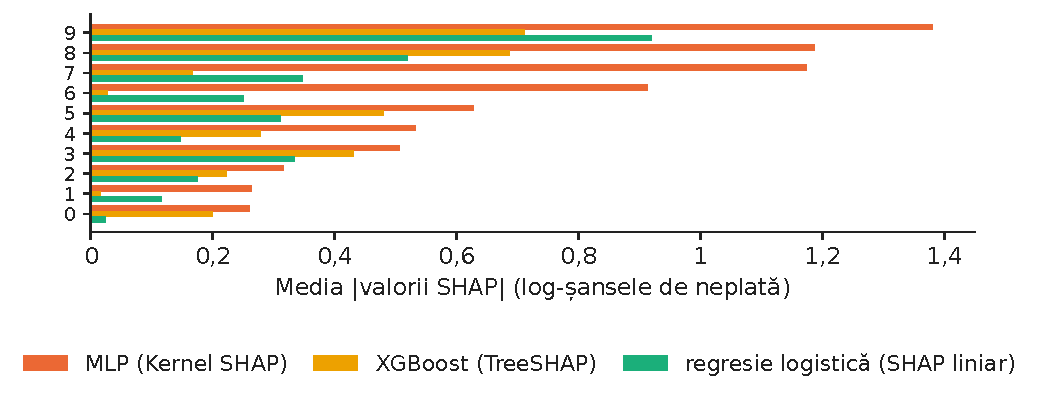
\includegraphics[width=\textwidth,height=0.265\textheight,keepaspectratio]{charts/ro/shap_global.pdf}\end{center}\vspace{-3mm}
\chartsource{Sursa: Baesens, Roesch și Scheule (2016), datele HMEQ. Date: 400 de solicitanți din test, 100 de solicitanți de referință.}
\vspace{0.5mm}
\begin{itemize}\setlength{\itemsep}{0pt}
  \item Pe primul loc la toate trei modelele: DEBTINC\_missing
    \begin{itemize}\setlength{\itemsep}{0pt}
      \item La MLP urmează DELINQ și JOB\_Other
      \item Corelația Spearman a importanțelor MLP--XGBoost 0{,}55, MLP--logistic 0{,}79.
    \end{itemize}
  \item Raportul datorie/venit (DEBTINC) lipsește la 21{,}3\,\% dintre credite
    \begin{itemize}\setlength{\itemsep}{0pt}
      \item Rata de neplată este 62{,}0\,\% cînd lipsește și 8{,}6\,\% cînd este raportat.
    \end{itemize}
\end{itemize}
\par\vfill\manager{o explicație poate arăta că modelul notează dosarul, nu debitorul
    \begin{itemize}\setlength{\itemsep}{0pt}
      \item Decideți dacă acest lucru este acceptabil.
    \end{itemize}}\par\vspace{0.5mm}
\par\vfill\noindent{\scriptsize\color{FooterGray}(calcul propriu)}\hfill\qlink{NN\_L11\_shap\_global}{Quantlets/L11/NN_L11_shap_global}\par\vspace{0.5mm}
\end{frame}

\begin{frame}{Diagrama roi: sensul și dispersia fiecărui efect}
\small
\intuition{fiecare punct este un solicitant; culoarea = rangul valorii variabilei; poziția = valoarea SHAP.}
\begin{center}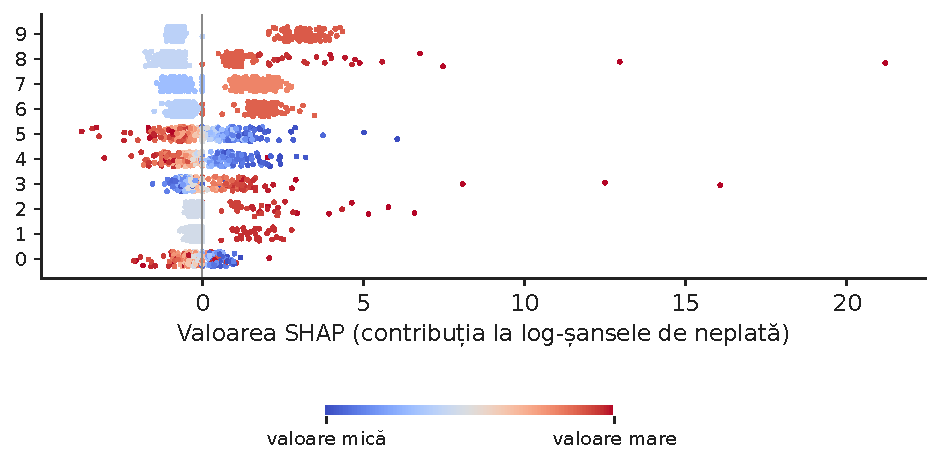
\includegraphics[width=\textwidth,height=0.539\textheight,keepaspectratio]{charts/ro/shap_beeswarm.pdf}\end{center}\vspace{-3mm}
\chartsource{Sursa: Baesens, Roesch și Scheule (2016), datele HMEQ. Date: 400 de solicitanți din test; culoarea = rangul valorii variabilei.}
\vspace{0.5mm}
\begin{itemize}\setlength{\itemsep}{0pt}
  \item Liniile de credit cu restanțe (DELINQ) și rapoartele negative (DEROG): valorile mari cresc riscul, așa cum se așteaptă în teoria creditului.
\end{itemize}
\par\vfill\noindent{\scriptsize\color{FooterGray}(calcul propriu)}\hfill\qlink{NN\_L11\_shap\_beeswarm}{Quantlets/L11/NN_L11_shap_beeswarm}\par\vspace{0.5mm}
\end{frame}

\begin{frame}{Explicația locală pentru un solicitant respins: diagrama cascadă SHAP}
\small
\intuition{de la log-șansele medii $\phi_0$ la scorul acestui solicitant, variabilă cu variabilă.}
\begin{center}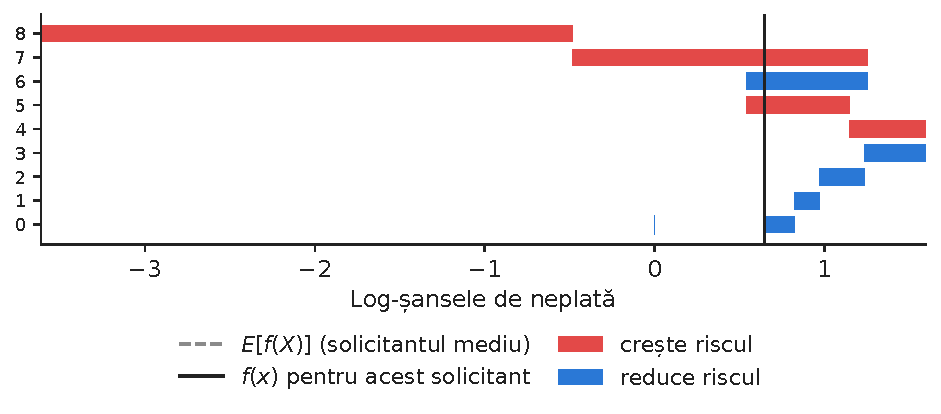
\includegraphics[width=\textwidth,height=0.426\textheight,keepaspectratio]{charts/ro/shap_waterfall.pdf}\end{center}\vspace{-3mm}
\chartsource{Sursa: Baesens, Roesch și Scheule (2016), datele HMEQ. Date: solicitant din test (rîndul 2411); valori în unitățile originale.}
\vspace{0.5mm}
\begin{itemize}\setlength{\itemsep}{0pt}
  \item Solicitant din test (rîndul 2411): PD 65{,}6\,\%, log-șanse 0{,}648 = \ensuremath{-}3{,}613 + 4{,}261
    \begin{itemize}\setlength{\itemsep}{0pt}
      \item Cele mai mari contribuții: DEBTINC\_missing (\ensuremath{+}3{,}13), JOB\_Other (\ensuremath{+}1{,}74), DELINQ (\ensuremath{-}0{,}71).
    \end{itemize}
\end{itemize}
\par\vfill\manager{notificarea de respingere enumeră principalele motive în această ordine, în cuvinte pe care clientul le înțelege.}\par\vspace{0.5mm}
\par\vfill\noindent{\scriptsize\color{FooterGray}(calcul propriu)}\hfill\qlink{NN\_L11\_shap\_waterfall}{Quantlets/L11/NN_L11_shap_waterfall}\par\vspace{0.5mm}
\end{frame}

\begin{frame}{Graficul de dependență: rețeaua a învățat semnalul valorii lipsă}
\small
\intuition{valoarea SHAP a DEBTINC în funcție de valoarea sa; punctele roșii sînt imputate cu mediana din antrenare.}
\begin{center}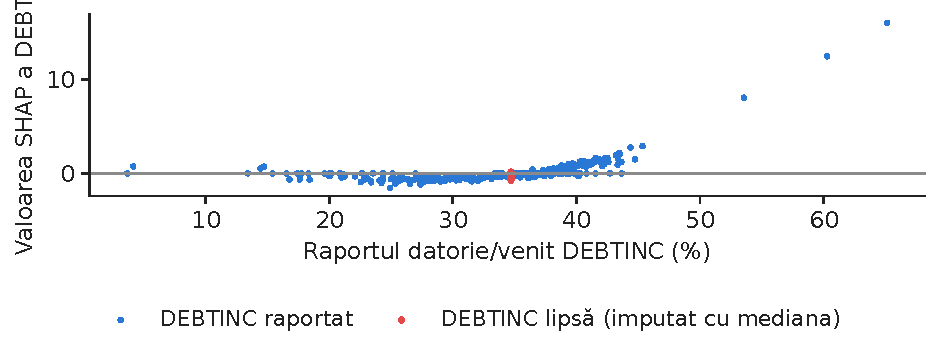
\includegraphics[width=\textwidth,height=0.369\textheight,keepaspectratio]{charts/ro/shap_dependence.pdf}\end{center}\vspace{-3mm}
\chartsource{Sursa: Baesens, Roesch și Scheule (2016), datele HMEQ. Date: 400 de solicitanți din test, MLP.}
\vspace{0.5mm}
\begin{itemize}\setlength{\itemsep}{0pt}
  \item Solicitanții cu valoare imputată au aceeași valoare DEBTINC
    \begin{itemize}\setlength{\itemsep}{0pt}
      \item Riscul lor este preluat de indicatorul de lipsă (SHAP mediu \ensuremath{+}3{,}13), nu de DEBTINC.
    \end{itemize}
\end{itemize}
\par\vfill\manager{alegerea metodei de imputare schimbă explicațiile
    \begin{itemize}\setlength{\itemsep}{0pt}
      \item Păstrați un indicator de lipsă pentru ca motivul să poată fi numit.
    \end{itemize}}\par\vspace{0.5mm}
\par\vfill\noindent{\scriptsize\color{FooterGray}(calcul propriu)}\hfill\qlink{NN\_L11\_shap\_dependence}{Quantlets/L11/NN_L11_shap_dependence}\par\vspace{0.5mm}
\end{frame}


\section{LIME, contrafactuale și efecte globale}

\begin{frame}{LIME: un model simplu, fidel în jurul unui punct}
\footnotesize
\intuition{solicitantul este perturbat, perturbările sînt ponderate după apropiere și se estimează un model liniar rar pe răspunsurile rețelei.}
\begin{columns}[T,onlytextwidth]
\begin{column}{0.56\textwidth}
\[ \xi(\vx)=\argmin_{g\in\mathcal{G}}\ \sum_{\vz}\pi_{\vx}(\vz)\big[f(\vz)-g(\vz)\big]^2+\Omega(g) \]\[ \pi_{\vx}(\vz)=\exp\!\Big(-\frac{\|\vz-\vx\|^2}{\sigma^2}\Big) \]{\footnotesize\begin{itemize}\setlength{\itemsep}{0pt}
  \item \textbf{\txtwhere}
    \begin{itemize}\setlength{\itemsep}{0pt}
      \item $\mathcal{G}$ = modelele liniare $g(\vz)=\beta_0+\boldsymbol\beta^{\top}\vz$
      \item $\Omega$ = penalizarea complexității
      \item $\vz\sim\mathcal{N}(\vx,\mathbf{I})$ în unități standardizate
      \item Lățimea nucleului $\sigma=0{,}75\sqrt{d}$ = 3{,}18 implicit.
    \end{itemize}
\end{itemize}\par}
\end{column}
\begin{column}{0.41\textwidth}
\begin{itemize}\setlength{\itemsep}{3pt}
  \item \textbf{Pantă locală}, nu o împărțire a prognozei: coeficienții nu se adună la $f(\vx)$.
  \item \textbf{Trei alegeri} decid rezultatul: vecinătatea, lățimea nucleului, numărul de eșantioane.
  \item \textbf{Solicitantul nostru}: variabila de top la LIME este DELINQ, la SHAP este DEBTINC\_missing.
\end{itemize}
\end{column}
\end{columns}
\par\vfill\manager{LIME răspunde la ``ce mișcă scorul în jurul acestui client?'', iar SHAP la ``de ce este acest client departe de medie?''.}\par\vspace{0.5mm}
\par\vfill\noindent{\scriptsize\color{FooterGray}(Ribeiro, Singh \& Guestrin, 2016)}\hfill\tryit{notebook \S3}\par\vspace{0.5mm}
\end{frame}

\begin{frame}{LIME și SHAP pentru același solicitant}
\small
\intuition{panta LIME înmulțită cu valoarea standardizată, alături de contribuția SHAP, pentru cele mai importante opt variabile SHAP.}
\begin{center}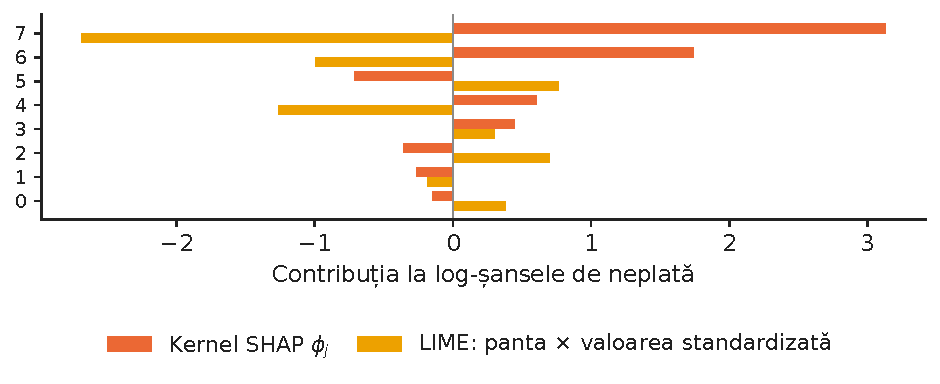
\includegraphics[width=\textwidth,height=0.500\textheight,keepaspectratio]{charts/ro/lime_vs_shap.pdf}\end{center}\vspace{-3mm}
\chartsource{Sursa: Baesens, Roesch și Scheule (2016), datele HMEQ. Date: solicitant din test (rîndul 2411); LIME cu 5 000 de eșantioane.}
\vspace{0.5mm}
\begin{itemize}\setlength{\itemsep}{0pt}
  \item Corelația Spearman a contribuțiilor absolute: 0{,}80
    \begin{itemize}\setlength{\itemsep}{0pt}
      \item Un indicator binar este departe de aproximarea sa liniară locală.
    \end{itemize}
\end{itemize}
\par\vfill\noindent{\scriptsize\color{FooterGray}(calcul propriu)}\hfill\qlink{NN\_L11\_lime\_vs\_shap}{Quantlets/L11/NN_L11_lime_vs_shap}\par\vspace{0.5mm}
\end{frame}

\begin{frame}{LIME depinde de propriile setări}
\small
\intuition{stînga: 30 de rulări cu valori inițiale diferite; dreapta: cele cinci pante cînd se schimbă lățimea nucleului.}
\begin{center}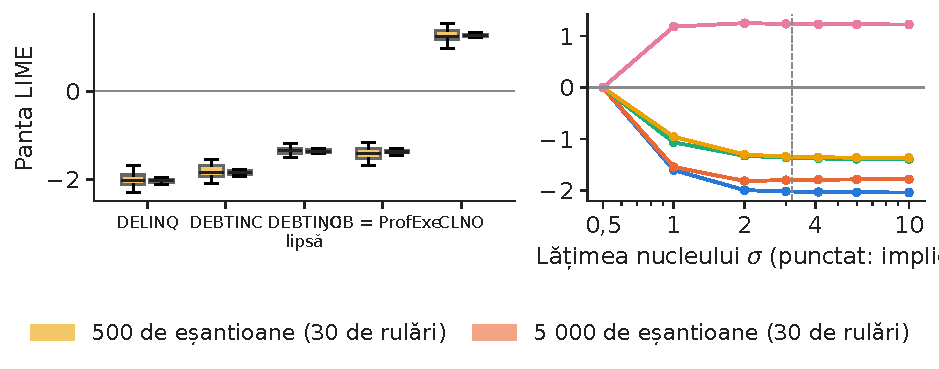
\includegraphics[width=\textwidth,height=0.310\textheight,keepaspectratio]{charts/ro/lime_instability.pdf}\end{center}\vspace{-3mm}
\chartsource{Sursa: Baesens, Roesch și Scheule (2016), datele HMEQ. Date: solicitant din test (rîndul 2411); dreapta: aceleași cinci variabile, 5 000 de eșantioane.}
\vspace{0.5mm}
\begin{itemize}\setlength{\itemsep}{0pt}
  \item Aceeași variabilă de top: 73\,\% din rulări cu 500 de eșantioane, 100\,\% cu 5 000
    \begin{itemize}\setlength{\itemsep}{0pt}
      \item Suprapunerea Jaccard a primelor 5 variabile 0{,}72, respectiv 1{,}00
      \item Coeficientul de variație 10\,\%, respectiv 2\,\%.
    \end{itemize}
\end{itemize}
\par\vfill\manager{fixați și raportați valoarea inițială, mărimea eșantionului și lățimea nucleului pentru orice explicație LIME care ajunge la un client sau la un auditor.}\par\vspace{0.5mm}
\par\vfill\noindent{\scriptsize\color{FooterGray}(calcul propriu)}\hfill\qlink{NN\_L11\_lime\_instability}{Quantlets/L11/NN_L11_lime_instability}\par\vspace{0.5mm}
\end{frame}

\begin{frame}{Explicații contrafactuale: ce ar trebui să se schimbe?}
\footnotesize
\intuition{se caută cel mai apropiat solicitant, schimbînd doar variabile acționabile, pe care modelul l-ar accepta.}
\begin{columns}[T,onlytextwidth]
\begin{column}{0.55\textwidth}
\[ \vx'=\argmin_{\vx'}\ \lambda\,\big(f(\vx')-t\big)_+^{2}+\sum_{j\in\mathcal{A}}\frac{|x'_j-x_j|}{\mathrm{MAD}_j} \]{\footnotesize\begin{itemize}\setlength{\itemsep}{0pt}
  \item \textbf{\txtwhere}
    \begin{itemize}\setlength{\itemsep}{0pt}
      \item $t$ = log-șansele-țintă ($-0{,}5$, sub pragul PD de 0{,}5)
      \item $\mathcal{A}$ = variabilele acționabile (LOAN, DEBTINC, NINQ, DELINQ, DEROG, CLNO, MORTDUE)
      \item Abaterea absolută mediană (MAD) scalează distanța
      \item Valorile brute rămîn $\ge0$, numărătorile sînt rotunjite.
    \end{itemize}
\end{itemize}\par}
\end{column}
\begin{column}{0.42\textwidth}
{\footnotesize\renewcommand{\arraystretch}{1.05}\setlength{\tabcolsep}{4pt}
\begin{tabular}{@{}lrr@{}}\toprule
Variabila & acum & necesar \\ \midrule
MORTDUE & 69\,115{,}0 & 57\,456{,}5 \\
DEBTINC & 34{,}7 & 33{,}4 \\
LOAN & 14\,500{,}0 & 15\,700{,}0 \\
\bottomrule\end{tabular}}\begin{itemize}\setlength{\itemsep}{1pt}
  \item PD 65{,}6\,\% $\to$ 39{,}2\,\% după aceste schimbări.
  \item Contrafactualul documentar: raportarea DEBTINC (la mediana 34{,}7) dă PD 5{,}1\,\%.
\end{itemize}
\end{column}
\end{columns}
\par\vfill\manager{``aduceți documentul de venit care lipsește'' este un răspuns mai bun pentru client decît orice listă de valori SHAP.}\par\vspace{0.5mm}
\par\vfill\noindent{\scriptsize\color{FooterGray}(Wachter, Mittelstadt \& Russell, 2017)}\hfill\tryit{notebook \S4}\par\vspace{0.5mm}
\end{frame}

\begin{frame}{Efecte globale: dependența parțială și ICE}
\small
\intuition{PDP mediază prognoza pe date cînd o variabilă este fixată la o valoare din grilă; ICE păstrează cîte o curbă pentru fiecare observație.}
\vspace{-1mm}\[ \mathrm{PD}_j(z)=\frac1n\sum_{i=1}^{n}f(z,\vx_{i,-j}),\qquad \mathrm{ICE}_{i,j}(z)=f(z,\vx_{i,-j}) \]\vspace{-2mm}
\begin{center}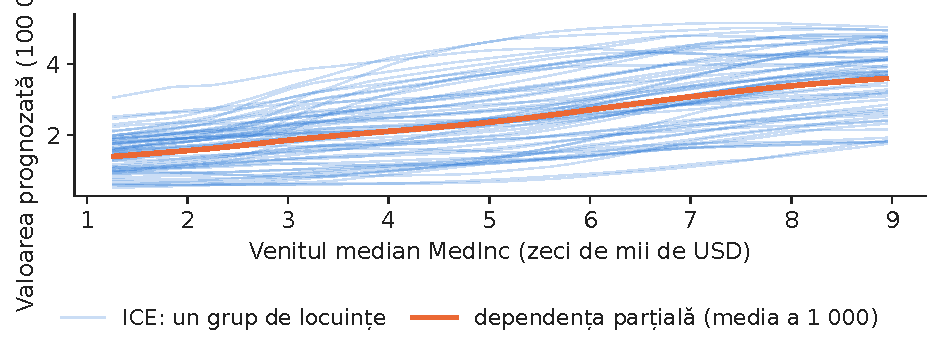
\includegraphics[width=\textwidth,height=0.318\textheight,keepaspectratio]{charts/ro/pdp_ice.pdf}\end{center}\vspace{-3mm}
\chartsource{Sursa: StatLib, locuințe din California, recensămîntul din 1990 (Pace și Barry, 1997). Date: MLP; 60 de grupuri de test (ICE), 1 000 pentru PDP.}
\vspace{0.5mm}
\begin{itemize}\setlength{\itemsep}{0pt}
  \item MLP pentru locuințele din California ($R^2$ de test 0{,}819, liniar 0{,}620): valoarea prognozată crește de la 1{,}40 la 3{,}60 (100 000 USD) pe grila de venit
    \begin{itemize}\setlength{\itemsep}{0pt}
      \item Dispersia curbelor ICE la capăt 0{,}95.
    \end{itemize}
\end{itemize}
\par\vfill\noindent{\scriptsize\color{FooterGray}(Friedman, 2001; Goldstein et al., 2015)}\hfill\qlink{NN\_L11\_pdp\_ice}{Quantlets/L11/NN_L11_pdp_ice}\par\vspace{0.5mm}
\end{frame}


\section{Metode bazate pe gradient pentru rețele neuronale}

\begin{frame}{Studiul de caz pentru fraudă: o rețea antrenată pe ziua 1, explicată pe ziua 2}
\footnotesize
\intuition{pentru o rețea gradienții sînt gratuiți: o singură trecere înapoi dă sensibilitatea scorului de fraudă la fiecare intrare.}
\begin{columns}[T,onlytextwidth]
\begin{column}{0.55\textwidth}
\[ \mathrm{saliency}_j(\vx)=\Big|\frac{\partial f(\vx)}{\partial x_j}\Big|,\qquad \mathrm{G\!\times\!I}_j(\vx)=(x_j-x'_j)\,\frac{\partial f(\vx)}{\partial x_j} \]{\footnotesize\begin{itemize}\setlength{\itemsep}{0pt}
  \item \textbf{\txtwhere}
    \begin{itemize}\setlength{\itemsep}{0pt}
      \item $f$ = log-șansele de fraudă ale unui MLP pe V1--V28 și logaritmul sumei
      \item $\vx'$ = referința = tranzacția legitimă medie din ziua 1
      \item Ponderea clasei $\sqrt{\text{dezechilibru}}$, oprire timpurie după PR-AUC ponderat de validare.
    \end{itemize}
\end{itemize}\par}
\end{column}
\begin{column}{0.42\textwidth}
\begin{itemize}\setlength{\itemsep}{3pt}
  \item \textbf{Test, ziua 2} (ponderi pentru datele complete): PR-AUC MLP 0{,}815, logistic 0{,}742
    \begin{itemize}\setlength{\itemsep}{0pt}
      \item AUC 0{,}961, respectiv 0{,}964.
    \end{itemize}
  \item \textbf{Saturarea}: într-o zonă plată a lui $f$ gradientul este aproape zero chiar și pentru o variabilă decisivă.
  \item \textbf{Rețelele ReLU}: gradientul este constant pe porțiuni, deci saliența sare între regiunile liniare.
\end{itemize}
\end{column}
\end{columns}
\par\vfill\manager{un analist de fraudă primește lista ordonată a intrărilor care au declanșat alerta, în milisecunde pe tranzacție.}\par\vspace{0.5mm}
\par\vfill\noindent{\scriptsize\color{FooterGray}(Simonyan, Vedaldi \& Zisserman, 2014; Dal Pozzolo et al., 2015)}\hfill\tryit{notebook \S5}\par\vspace{0.5mm}
\end{frame}

\begin{frame}{Gradienții integrați: atribuiri care se adună}
\footnotesize
\intuition{se integrează gradientul pe drumul drept de la referință la intrare; atribuirile se adună la $f(\vx)-f(\vx')$.}
\begin{columns}[T,onlytextwidth]
\begin{column}{0.6\textwidth}
\[ \mathrm{IG}_j(\vx)=(x_j-x'_j)\int_0^1\frac{\partial f\big(\vx'+\alpha(\vx-\vx')\big)}{\partial x_j}\,d\alpha \]\[ \approx(x_j-x'_j)\frac1m\sum_{k=1}^{m}\frac{\partial f\big(\vx'+\tfrac{k-1/2}{m}(\vx-\vx')\big)}{\partial x_j} \]{\footnotesize\begin{itemize}\setlength{\itemsep}{0pt}
  \item \textbf{\txtwhere}
    \begin{itemize}\setlength{\itemsep}{0pt}
      \item $m$ = pașii Riemann (regula punctului de mijloc, 64 aici)
      \item Completitudinea $\sum_j\mathrm{IG}_j=f(\vx)-f(\vx')$ rezultă din teorema fundamentală a calculului integral pe drumuri.
    \end{itemize}
\end{itemize}\par}
\end{column}
\begin{column}{0.37\textwidth}
\begin{itemize}\setlength{\itemsep}{3pt}
  \item \textbf{Axiome} (Sundararajan et al., 2017)
    \begin{itemize}\setlength{\itemsep}{0pt}
      \item Completitudinea; sensibilitatea: o variabilă care schimbă $f$ primește o atribuire nenulă
      \item Invarianța la implementare: funcții egale, atribuiri egale
    \end{itemize}
  \item \textbf{Legătura cu Shapley}: IG este valoarea Aumann-Shapley a jocului continuu de-a lungul drumului.
  \item \textbf{Referința contează}: ``tranzacția legitimă medie'' răspunde la ``de ce nu este aceasta o plată normală?''.
\end{itemize}
\end{column}
\end{columns}
\par\vfill\manager{scrieți referința în documentația modelului: o altă referință înseamnă o altă întrebare.}\par\vspace{0.5mm}
\par\vfill\noindent{\scriptsize\color{FooterGray}(Sundararajan, Taly \& Yan, 2017)}\hfill\tryit{notebook \S5}\par\vspace{0.5mm}
\end{frame}

\begin{frame}{Completitudinea se verifică atunci cînd integrala este calculată precis}
\small
\intuition{mediana lui $|\sum_j\mathrm{IG}_j-(f(\vx)-f(\vx'))|/|f(\vx)-f(\vx')|$ pe fraudele din ziua 2.}
\begin{center}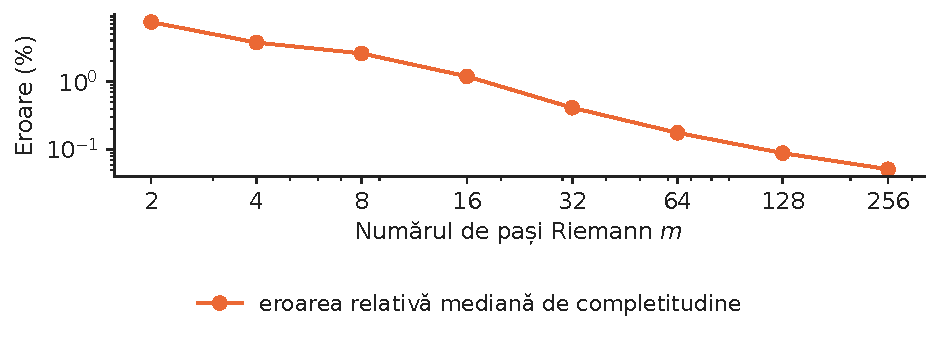
\includegraphics[width=\textwidth,height=0.500\textheight,keepaspectratio]{charts/ro/ig_completeness.pdf}\end{center}\vspace{-3mm}
\chartsource{Sursa: ULB Machine Learning Group și Worldline, tranzacții cu carduri (OpenML 1597). Date: 211 fraude din ziua a doua; referința = tranzacția legitimă medie din ziua întîi.}
\vspace{0.5mm}
\begin{itemize}\setlength{\itemsep}{0pt}
  \item Eroare de 3{,}7\,\% cu 4 pași și de 0{,}18\,\% cu 64, pe 211 de fraude
    \begin{itemize}\setlength{\itemsep}{0pt}
      \item Eroarea scade aproximativ ca $1/m^{2}$, ca la regula punctului de mijloc.
    \end{itemize}
\end{itemize}
\par\vfill\noindent{\scriptsize\color{FooterGray}(calcul propriu)}\hfill\qlink{NN\_L11\_ig\_completeness}{Quantlets/L11/NN_L11_ig_completeness}\par\vspace{0.5mm}
\end{frame}

\begin{frame}{SmoothGrad și explicațiile la nivel de concept}
\footnotesize
\intuition{se mediază gradienții pe copii perturbate ale intrării pentru a elimina oscilațiile ReLU; sau se testează dacă un concept uman mișcă ieșirea.}
\begin{columns}[T,onlytextwidth]
\begin{column}{0.58\textwidth}
\[ \mathrm{SG}_j(\vx)=\frac1n\sum_{k=1}^{n}\frac{\partial f(\vx+\boldsymbol\varepsilon_k)}{\partial x_j},\quad \boldsymbol\varepsilon_k\sim\mathcal{N}(\mathbf 0,s^{2}\mathbf I) \]\[ S_{C}(\vx)=\nabla h(\vx)^{\top}\mathbf{v}_C \]{\footnotesize\begin{itemize}\setlength{\itemsep}{0pt}
  \item \textbf{\txtwhere}
    \begin{itemize}\setlength{\itemsep}{0pt}
      \item $n=50$, $s=0{,}15$ abateri standard
      \item Testarea cu vectori de activare a conceptelor (TCAV): $\mathbf{v}_C$ = normala unui clasificator liniar care separă exemplele conceptului $C$ într-un strat ascuns $h$
      \item Scorul TCAV este ponderea intrărilor cu $S_C>0$.
    \end{itemize}
\end{itemize}\par}
\end{column}
\begin{column}{0.39\textwidth}
\begin{itemize}\setlength{\itemsep}{3pt}
  \item \textbf{SmoothGrad} clarifică hărțile de saliență ale imaginilor și stabilizează gradienții tabelari (secțiunea următoare).
  \item \textbf{TCAV} vorbește limbajul afacerii: ``tranzacție de noapte'', ``comerciant nou'' --- dacă asemenea concepte sînt etichetate.
  \item \textbf{Datele noastre}: V1--V28 sînt componente anonimizate, deci aici nu se pot face teste pe concepte.
\end{itemize}
\end{column}
\end{columns}
\par\vfill\manager{explicațiile pe concepte cer concepte etichetate încă de la colectarea datelor.}\par\vspace{0.5mm}
\par\vfill\noindent{\scriptsize\color{FooterGray}(Smilkov et al., 2017; Kim et al., 2018)}\par\vspace{0.5mm}
\end{frame}

\begin{frame}{Patru metode de explicare aplicate unei tranzacții frauduloase}
\small
\intuition{atribuirile cu semn pentru o fraudă din ziua 2 (scorul median al fraudelor), ca ponderi în atribuirea absolută totală.}
\begin{center}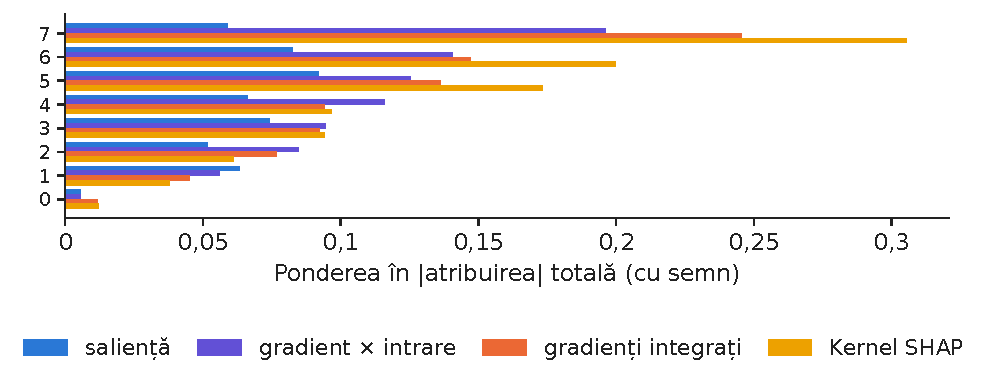
\includegraphics[width=\textwidth,height=0.481\textheight,keepaspectratio]{charts/ro/fraud_local.pdf}\end{center}\vspace{-3mm}
\chartsource{Sursa: ULB Machine Learning Group și Worldline, tranzacții cu carduri (OpenML 1597). Date: o fraudă din ziua a doua (scorul median al fraudelor).}
\vspace{0.5mm}
\begin{itemize}\setlength{\itemsep}{0pt}
  \item Variabila de top: Kernel SHAP V14, gradienți integrați V14, saliență V12
    \begin{itemize}\setlength{\itemsep}{0pt}
      \item Scorul de fraudă 99{,}9\,\%: saliența nu ține cont de mărimea abaterii față de referință.
    \end{itemize}
\end{itemize}
\par\vfill\noindent{\scriptsize\color{FooterGray}(calcul propriu)}\hfill\qlink{NN\_L11\_fraud\_local}{Quantlets/L11/NN_L11_fraud_local}\par\vspace{0.5mm}
\end{frame}


\section{Concordanța, fidelitatea și stabilitatea explicațiilor}

\begin{frame}{Concordanța metodelor: ridicată, dar nu perfectă}
\small
\intuition{corelația Spearman a importanțelor globale (media $|$atribuirii$|$) pentru șapte metode, pe aceleași fraude.}
\begin{center}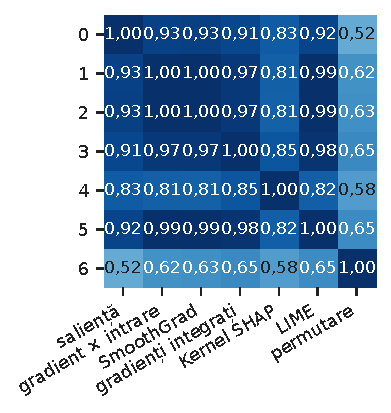
\includegraphics[width=\textwidth,height=0.348\textheight,keepaspectratio]{charts/ro/method_agreement.pdf}\end{center}\vspace{-3mm}
\chartsource{Sursa: ULB Machine Learning Group și Worldline, tranzacții cu carduri (OpenML 1597). Date: corelația Spearman a importanțelor globale; 211 fraude din ziua a doua.}
\vspace{0.5mm}
\begin{itemize}\setlength{\itemsep}{0pt}
  \item IG--SHAP 0{,}85, saliență--SHAP 0{,}83, LIME--SHAP 0{,}82, permutare--SHAP 0{,}58
    \begin{itemize}\setlength{\itemsep}{0pt}
      \item Toate metodele pun V12 pe primul loc.
    \end{itemize}
\end{itemize}
\par\vfill\manager{dezacordul este informație: importanța prin permutare arată de ce are nevoie modelul, atribuirile arată ce folosește.}\par\vspace{0.5mm}
\par\vfill\noindent{\scriptsize\color{FooterGray}(Breiman, 2001; calcul propriu)}\hfill\qlink{NN\_L11\_method\_agreement}{Quantlets/L11/NN_L11_method_agreement}\par\vspace{0.5mm}
\end{frame}

\begin{frame}{Fidelitatea explicațiilor: testul eliminării variabilelor}
\small
\intuition{variabilele de top $k$ ale fiecărei fraude sînt readuse la referință; o explicație fidelă face scorul să scadă repede.}
\vspace{-1mm}\[ \mathrm{AOPC}=\frac{1}{K}\sum_{k=1}^{K}\big[f(\vx)-f(\vx^{(k)})\big] \]\vspace{-2mm}
\begin{center}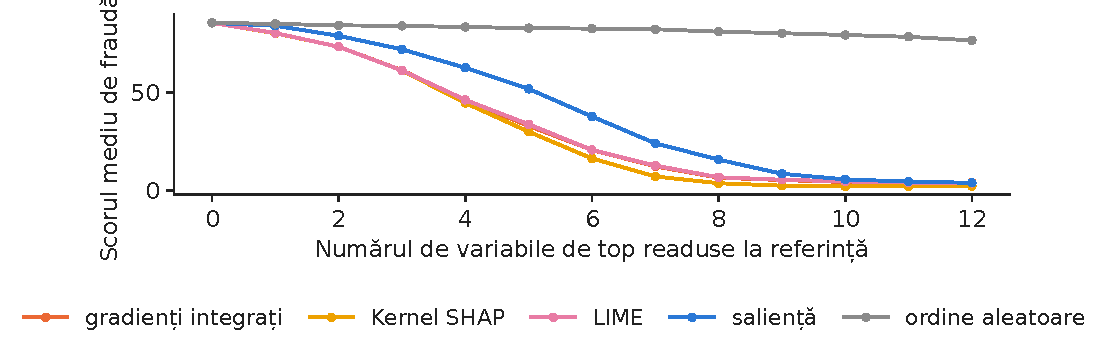
\includegraphics[width=\textwidth,height=0.371\textheight,keepaspectratio]{charts/ro/deletion_curve.pdf}\end{center}\vspace{-3mm}
\chartsource{Sursa: ULB Machine Learning Group și Worldline, tranzacții cu carduri (OpenML 1597). Date: 211 fraude din ziua a doua.}
\vspace{0.5mm}
\begin{itemize}\setlength{\itemsep}{0pt}
  \item Aria de deasupra curbei de perturbare (AOPC), în puncte de scor de fraudă: IG 56{,}2, SHAP 58{,}4, LIME 56{,}1, saliență 48{,}0, ordine aleatoare 3{,}9.
\end{itemize}
\par\vfill\noindent{\scriptsize\color{FooterGray}(Samek et al., 2017)}\hfill\qlink{NN\_L11\_deletion\_curve}{Quantlets/L11/NN_L11_deletion_curve}\par\vspace{0.5mm}
\end{frame}

\begin{frame}{Robustețea locală a explicațiilor la mici modificări ale intrării}
\small
\intuition{variația relativă a vectorului de atribuiri pe unitatea unei perturbări mici (raport de tip Lipschitz).}
\vspace{-1mm}\[ \hat L(\vx)=\frac{\|\mathbf a(\vx+\boldsymbol\varepsilon)-\mathbf a(\vx)\|/\|\mathbf a(\vx)\|}{\|\boldsymbol\varepsilon\|},\quad \boldsymbol\varepsilon\sim\mathcal N(\mathbf 0,0.05^{2}\mathbf I) \]\vspace{-2mm}
\begin{center}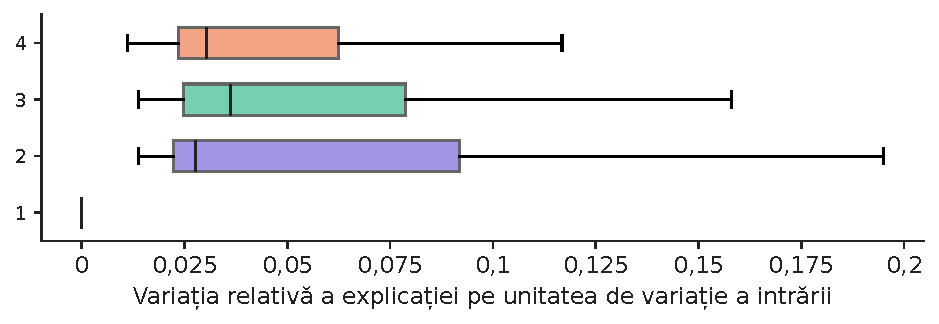
\includegraphics[width=\textwidth,height=0.384\textheight,keepaspectratio]{charts/ro/local_robustness.pdf}\end{center}\vspace{-3mm}
\chartsource{Sursa: ULB Machine Learning Group și Worldline, tranzacții cu carduri (OpenML 1597). Date: 60 de fraude din ziua a doua x 10 perturbări (sigma = 0,05 abateri standard).}
\vspace{0.5mm}
\begin{itemize}\setlength{\itemsep}{0pt}
  \item Mediane: saliență 0{,}000, gradient $\times$ intrare 0{,}028, IG 0{,}030, SmoothGrad 0{,}036
    \begin{itemize}\setlength{\itemsep}{0pt}
      \item În interiorul unei regiuni liniare a unei rețele ReLU gradientul nu se schimbă.
    \end{itemize}
\end{itemize}
\par\vfill\noindent{\scriptsize\color{FooterGray}(Alvarez-Melis \& Jaakkola, 2018)}\hfill\qlink{NN\_L11\_local\_robustness}{Quantlets/L11/NN_L11_local_robustness}\par\vspace{0.5mm}
\end{frame}

\begin{frame}{Efectul Rashomon: modele la fel de precise, cu explicații diferite}
\small
\intuition{rangul fiecărei variabile după media $|$SHAP$|$ pentru 10 rețele și 10 ansambluri de arbori reantrenate (doar valorile inițiale diferă).}
\begin{center}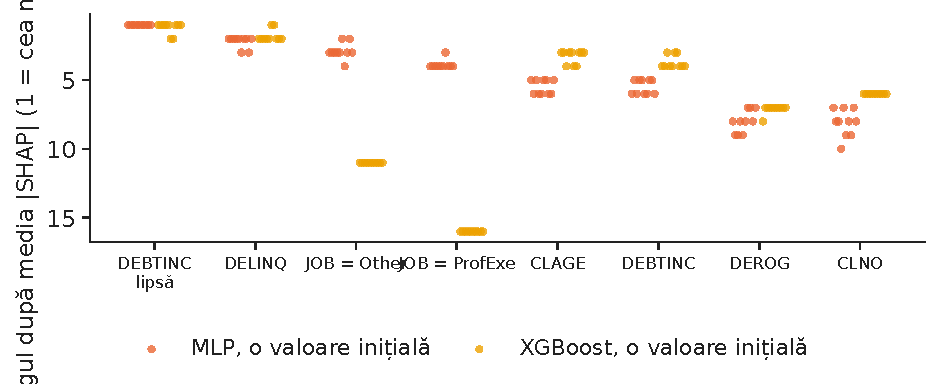
\includegraphics[width=\textwidth,height=0.374\textheight,keepaspectratio]{charts/ro/seed_stability.pdf}\end{center}\vspace{-3mm}
\chartsource{Sursa: Baesens, Roesch și Scheule (2016), datele HMEQ. Date: 10 valori inițiale de antrenare; 200 de solicitanți din test.}
\vspace{0.5mm}
\begin{itemize}\setlength{\itemsep}{0pt}
  \item AUC de test MLP între 0{,}929 și 0{,}941
    \begin{itemize}\setlength{\itemsep}{0pt}
      \item Tau Kendall mediu pe perechi (acordul rangurilor importanțelor, 1 = aceeași ordine): MLP 0{,}83, XGBoost 0{,}97
      \item Aceeași variabilă de top pentru un solicitant în 78\,\% (MLP) și 83\,\% (XGBoost) dintre perechile de valori inițiale.
    \end{itemize}
\end{itemize}
\par\vfill\noindent{\scriptsize\color{FooterGray}(calcul propriu)}\hfill\qlink{NN\_L11\_seed\_stability}{Quantlets/L11/NN_L11_seed_stability}\par\vspace{0.5mm}
\end{frame}

\begin{frame}{Explicațiile în timp: ziua 1 față de ziua 2}
\small
\intuition{ponderea în $|$IG$|$ total pe variabile, pentru fraudele rezervate din ziua de antrenare și pentru fraudele din ziua următoare.}
\begin{center}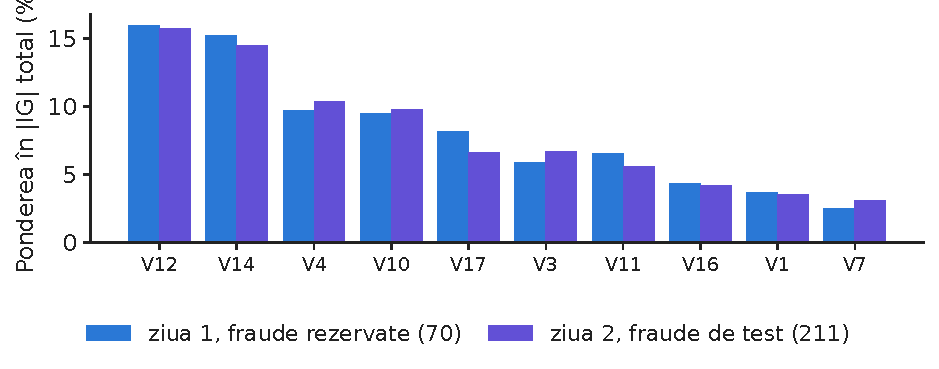
\includegraphics[width=\textwidth,height=0.286\textheight,keepaspectratio]{charts/ro/time_shift.pdf}\end{center}\vspace{-3mm}
\chartsource{Sursa: ULB Machine Learning Group și Worldline, tranzacții cu carduri (OpenML 1597). Date: model antrenat pe ziua 1; gradienți integrați.}
\vspace{0.5mm}
\begin{itemize}\setlength{\itemsep}{0pt}
  \item Spearman 0{,}98, divergența Jensen-Shannon (JS) (construită pe divergența Kullback-Leibler (KL)) 0{,}003, 4 variabile comune în primele 5
    \begin{itemize}\setlength{\itemsep}{0pt}
      \item După o zi, explicația este stabilă aici.
    \end{itemize}
\end{itemize}
\par\vfill\manager{monitorizați lunar distribuția atribuirilor, alături de distribuția scorurilor
    \begin{itemize}\setlength{\itemsep}{0pt}
      \item O deplasare a motivelor poate preceda o scădere a acurateței.
    \end{itemize}}\par\vspace{0.5mm}
\par\vfill\noindent{\scriptsize\color{FooterGray}(calcul propriu)}\hfill\qlink{NN\_L11\_time\_shift}{Quantlets/L11/NN_L11_time_shift}\par\vspace{0.5mm}
\end{frame}

\begin{frame}{Fișa de stabilitate a acestui curs}
\small
{\footnotesize\renewcommand{\arraystretch}{1.05}\setlength{\tabcolsep}{4pt}
\begin{tabular}{@{}p{0.3\textwidth}p{0.32\textwidth}p{0.3\textwidth}@{}}\toprule
Sursa schimbării & Măsura & Rezultat \\ \midrule
Aleatorismul explicației (LIME) & aceeași variabilă de top în 30 de rulări & 73\,\% (500), 100\,\% (5 000 de eșantioane) \\
Valoarea inițială (Rashomon) & tau Kendall al importanțelor globale & MLP 0{,}83, XGBoost 0{,}97 \\
Valoarea inițială, un solicitant & aceeași variabilă de top & MLP 78\,\%, XGBoost 83\,\% \\
Metoda & Spearman al importanțelor & 0{,}52 -- 1{,}00 \\
Zgomotul la intrare & variația relativă mediană & IG 0{,}030, SmoothGrad 0{,}036 \\
Timpul (ziua 1 $\to$ ziua 2) & Spearman, divergența JS & 0{,}98; 0{,}003 \\
\bottomrule\end{tabular}}
\par\vfill\manager{raportați orice explicație împreună cu stabilitatea ei: ce valoare inițială, ce eșantion, ce perioadă și cît se modifică.}\par\vspace{0.5mm}
\par\vfill\noindent{\scriptsize\color{FooterGray}(calcul propriu)}\par\vspace{0.5mm}
\end{frame}


\section{Explicabilitatea în guvernanța modelelor}

\begin{frame}{Lista de verificare pentru un audit al explicabilității}
\small
\begin{columns}[T,onlytextwidth]
\begin{column}{0.49\textwidth}
\begin{itemize}\setlength{\itemsep}{4pt}
  \item \textbf{Scopul}: cine citește explicația (client, analist, validator, autoritate) și ce decizie susține.
  \item \textbf{Setările}: eșantionul de referință, referința, valoarea inițială, numărul de eșantioane, lățimea nucleului --- versionate odată cu modelul.
  \item \textbf{Verificările}: aditivitate/completitudine, fidelitate (eliminare), stabilitate (valori inițiale, timp), concordanța a două metode.
\end{itemize}
\end{column}
\begin{column}{0.49\textwidth}
\begin{itemize}\setlength{\itemsep}{4pt}
  \item \textbf{Echitatea}: atribuirile variabilelor protejate și ale substitutelor lor (vîrstă, sex, cod poștal)
    \begin{itemize}\setlength{\itemsep}{0pt}
      \item O explicație arată utilizarea, nu cauzalitatea.
    \end{itemize}
  \item \textbf{Pentru client}: puține motive, contrafactuale acționabile, fără nume brute de componente (V14 nu înseamnă nimic pentru un client).
  \item \textbf{Alternativa}: dacă un model interpretabil este aproape la fel de precis (aici AUC logistic 0{,}909 față de MLP 0{,}935), luați-l în considerare.
\end{itemize}
\end{column}
\end{columns}
\par\vfill\manager{raportul de validare trebuie să conțină explicațiile și testele lor de stabilitate, nu doar acuratețea.}\par\vspace{0.5mm}
\par\vfill\noindent{\scriptsize\color{FooterGray}(SR 11-7; Rudin, 2019)}\par\vspace{0.5mm}
\end{frame}

\section*{Recapitulare}

\begin{frame}{Test 1: adunarea valorilor SHAP}
\small
\begin{itemize}
  \item Pentru solicitantul nostru valoarea de bază este \ensuremath{-}3{,}613, iar valorile SHAP se adună la 4{,}261.
    \begin{itemize}\setlength{\itemsep}{0pt}
      \item Care sînt log-șansele de neplată date de model și de ce sînteți siguri?
    \end{itemize}
\end{itemize}
\vspace{2mm}
\begin{exampleblock}{R\u{a}spuns}
\begin{itemize}
  \item 0{,}648: din axioma eficienței, $f(\vx)=\phi_0+\sum_j\phi_j$
    \begin{itemize}\setlength{\itemsep}{0pt}
      \item PD este $\sigma$(0{,}648) = 65{,}6\,\%.
    \end{itemize}
\end{itemize}
\end{exampleblock}
\end{frame}

\begin{frame}{Test 2: un LIME instabil}
\small
\begin{itemize}
  \item Doi analiști explică același solicitant respins cu LIME și raportează motive principale diferite.
    \begin{itemize}\setlength{\itemsep}{0pt}
      \item Este modelul inconsecvent?
    \end{itemize}
\end{itemize}
\vspace{2mm}
\begin{exampleblock}{R\u{a}spuns}
\begin{itemize}
  \item Nu neapărat: LIME eșantionează perturbări
    \begin{itemize}\setlength{\itemsep}{0pt}
      \item Cu 500 de eșantioane variabila de top a coincis în 73\,\% din rulările noastre
      \item Fixați valoarea inițială, creșteți eșantionul, comparați cu SHAP.
    \end{itemize}
\end{itemize}
\end{exampleblock}
\end{frame}

\begin{frame}{Test 3: alegerea referinței IG}
\small
\begin{itemize}
  \item Un coleg folosește vectorul nul ca referință pentru gradienții integrați, pe variabile de fraudă standardizate.
    \begin{itemize}\setlength{\itemsep}{0pt}
      \item La ce întrebare răspunde explicația?
    \end{itemize}
\end{itemize}
\vspace{2mm}
\begin{exampleblock}{R\u{a}spuns}
\begin{itemize}
  \item ``De ce diferă această tranzacție de tranzacția medie (inclusiv fraudele)?''
    \begin{itemize}\setlength{\itemsep}{0pt}
      \item Referința noastră, tranzacția legitimă medie, întreabă de ce nu este o plată normală.
    \end{itemize}
\end{itemize}
\end{exampleblock}
\end{frame}

\begin{frame}{Recapitulare}
\small
\begin{itemize}\setlength{\itemsep}{4pt}
  \item \textbf{SHAP}: valori Shapley cu verificarea exactă a aditivității
    \begin{itemize}\setlength{\itemsep}{0pt}
      \item Lipsa raportului datorie/venit determină rețeaua de credit.
    \end{itemize}
  \item \textbf{LIME}: o pantă locală care depinde de valoarea inițială, de eșantion și de lățimea nucleului
    \begin{itemize}\setlength{\itemsep}{0pt}
      \item Utilă, dar raportați setările.
    \end{itemize}
  \item \textbf{Gradienți}: gradienții integrați satisfac completitudinea (eroare de 0{,}18\,\% la 64 de pași) și sînt la fel de fideli ca SHAP, la un cost mult mai mic.
  \item \textbf{Stabilitatea}: reantrenarea cu altă valoare inițială reordonează variabilele (tau Kendall 0{,}83 pentru MLP)
    \begin{itemize}\setlength{\itemsep}{0pt}
      \item Explicațiile trebuie testate ca modelele.
    \end{itemize}
  \item \textbf{Urmează}: cursul 12, modelele lingvistice mari, unde explicațiile devin text.
\end{itemize}
\end{frame}

\begin{frame}{Cercetările grupului nostru: XAI în fraudă și piețele de energie}
\footnotesize
\begin{itemize}\setlength{\itemsep}{4pt}
  \item \textbf{Stabilitatea SHAP în detectarea fraudei cu informație din graf}: pe datele de fraudă IEEE-CIS se compară contribuțiile SHAP ale unui model XGBoost cu reprezentări dintr-o rețea neuronală pe grafuri (GNN), sub validare aleatoare și validare înainte în timp, cu un control gaussian de aceeași dimensiune și covarianță
    \begin{itemize}\setlength{\itemsep}{0pt}
      \item Dacă modelul cu graf pare mai stabil depinde de modul în care se măsoară schimbarea, un protocol riguros pentru stabilitatea explicațiilor (Diaconu \& Pele, 2026, trimis la Expert Systems with Applications; cod: QuantLet GNN\_XAI\_Stability).
    \end{itemize}
  \item \textbf{Avertizarea timpurie explicabilă a vîrfurilor de preț} la energia electrică din România (Andrei, Pele, Cramer, Amza \& Diaconu, 2026, Proceedings of the International Conference on Business Excellence (PICBE)) și \textbf{detectarea anomaliilor de preț cu SHAP} (Andrei \& Pele, 2025, Preprints).
  \item \textbf{Explicabilitatea pe mai multe orizonturi} a prognozelor de preț: ce factori contează la fiecare orizont pe piața liberalizată din România (Andrei, Pele \& Cramer, 2026, PICBE).
\end{itemize}\par\vspace{1mm}{\scriptsize \begin{itemize}
  \item Rezultatele sînt cele din lucrări; cifrele de pe celelalte slide-uri provin din datele noastre.
\end{itemize}}
\par\vfill\noindent{\scriptsize\color{FooterGray}(Academia de Studii Economice din București (ASE); Academia Română, Institutul de Prognoză Economică (IPE))}\par\vspace{0.5mm}
\end{frame}

\begin{frame}{Lecturi și resurse suplimentare}
\small
\begin{columns}[T,onlytextwidth]
\begin{column}{0.5\textwidth}
\begin{itemize}\setlength{\itemsep}{4pt}
  \item \textbf{C.\ Molnar, Interpretable Machine Learning}, gratuit online: \href{https://christophm.github.io/interpretable-ml-book/}{christophm.github.io/interpretable-ml-book}.
  \item \textbf{Biblioteca SHAP} și exemple: \href{https://shap.readthedocs.io}{shap.readthedocs.io}.
  \item \textbf{Rudin (2019)}: argumentele pentru modele interpretabile în deciziile cu miză mare.
\end{itemize}
\end{column}
\begin{column}{0.47\textwidth}
\begin{itemize}\setlength{\itemsep}{4pt}
  \item \textbf{Acest curs}: cod, date, notebook-uri --- \href{https://github.com/danpele/NEURAL_BIZ}{github.com/danpele/NEURAL\_BIZ}.
  \item \textbf{Încercați singuri}: notebooks/L11\_notebook\_ro.ipynb
    \begin{itemize}\setlength{\itemsep}{0pt}
      \item Seminarul explică un model pentru German credit, cu o verificare a echității.
    \end{itemize}
  \item \textbf{Replicarea studiului nostru de stabilitate}: \href{https://github.com/QuantLet/GNN_XAI_Stability}{github.com/QuantLet/GNN\_XAI\_Stability}.
\end{itemize}
\end{column}
\end{columns}
\end{frame}

\begin{frame}{Bibliografie (1/3)}
\scriptsize
\begin{itemize}\setlength{\itemsep}{0pt}\scriptsize
\item Alvarez-Melis, D.\ \& Jaakkola, T.\,S.\ (2018). On the robustness of interpretability methods. ICML Workshop on Human Interpretability in Machine Learning. \href{https://arxiv.org/abs/1806.08049}{arXiv:1806.08049}
\item Andrei, A.-V.\ \& Pele, D.\,T.\ (2025). Explainable AI for electricity price anomaly detection: A SHAP-driven approach in Romania's energy market. \textit{Preprints}. \href{https://doi.org/10.20944/preprints202508.0410.v1}{doi:10.20944/preprints202508.0410.v1}
\item Andrei, A.-V., Pele, D.-T.\ \& Cramer, A.-A.\ (2026). Multi-horizon explainability in energy price forecasting: Disentangling market dynamics and renewable intermittency in Romania's liberalized electricity market. \textit{Proceedings of the International Conference on Business Excellence}, 20(1), 104--117. \href{https://doi.org/10.2478/picbe-2026-0014}{doi:10.2478/picbe-2026-0014}
\item Andrei, A.-V., Pele, D.-T., Cramer, A.-A., Amza, A.\ \& Diaconu, D.\ (2026). Explainable AI-based early warning system for electricity price spikes: Evidence from the Romanian market. \textit{Proceedings of the International Conference on Business Excellence}, 20(1), 4820--4836. \href{https://doi.org/10.2478/picbe-2026-0352}{doi:10.2478/picbe-2026-0352}
\item Baesens, B., Roesch, D.\ \& Scheule, H.\ (2016). \textit{Credit Risk Analytics: Measurement Techniques, Applications, and Examples in SAS}. Wiley.
\item Breiman, L.\ (2001). Random forests. \textit{Machine Learning}, 45, 5--32. \href{https://doi.org/10.1023/A:1010933404324}{doi:10.1023/A:1010933404324}
\item Dal Pozzolo, A., Caelen, O., Johnson, R.\,A.\ \& Bontempi, G.\ (2015). Calibrating probability with undersampling for unbalanced classification. IEEE SSCI, 159--166. \href{https://doi.org/10.1109/SSCI.2015.33}{doi:10.1109/SSCI.2015.33}
\item Diaconu, D.\ \& Pele, D.\,T.\ (2026). SHAP stability across random and forward-time validation in graph-augmented fraud detection. Submitted to \textit{Expert Systems with Applications}. Code: \href{https://github.com/QuantLet/GNN_XAI_Stability}{github.com/QuantLet/GNN\_XAI\_Stability}
\end{itemize}
\end{frame}

\begin{frame}{Bibliografie (2/3)}
\scriptsize
\begin{itemize}\setlength{\itemsep}{0pt}\scriptsize
\item Friedman, J.\,H.\ (2001). Greedy function approximation: A gradient boosting machine. \textit{Annals of Statistics}, 29(5), 1189--1232. \href{https://doi.org/10.1214/aos/1013203451}{doi:10.1214/aos/1013203451}
\item Goldstein, A., Kapelner, A., Bleich, J.\ \& Pitkin, E.\ (2015). Peeking inside the black box: Visualizing statistical learning with plots of individual conditional expectation. \textit{Journal of Computational and Graphical Statistics}, 24(1), 44--65. \href{https://doi.org/10.1080/10618600.2014.907095}{doi:10.1080/10618600.2014.907095}
\item Kim, B.\ et al.\ (2018). Interpretability beyond feature attribution: Quantitative testing with concept activation vectors (TCAV). ICML. \href{https://arxiv.org/abs/1711.11279}{arXiv:1711.11279}
\item Lundberg, S.\,M.\ \& Lee, S.-I.\ (2017). A unified approach to interpreting model predictions. \textit{Advances in Neural Information Processing Systems}, 30. \href{https://arxiv.org/abs/1705.07874}{arXiv:1705.07874}
\item Lundberg, S.\,M.\ et al.\ (2020). From local explanations to global understanding with explainable AI for trees. \textit{Nature Machine Intelligence}, 2, 56--67. \href{https://doi.org/10.1038/s42256-019-0138-9}{doi:10.1038/s42256-019-0138-9}
\item Ribeiro, M.\,T., Singh, S.\ \& Guestrin, C.\ (2016). ``Why should I trust you?'' Explaining the predictions of any classifier. KDD, 1135--1144. \href{https://doi.org/10.1145/2939672.2939778}{doi:10.1145/2939672.2939778}
\item Rudin, C.\ (2019). Stop explaining black box machine learning models for high stakes decisions and use interpretable models instead. \textit{Nature Machine Intelligence}, 1, 206--215. \href{https://doi.org/10.1038/s42256-019-0048-x}{doi:10.1038/s42256-019-0048-x}
\item Samek, W., Binder, A., Montavon, G., Lapuschkin, S.\ \& Müller, K.-R.\ (2017). Evaluating the visualization of what a deep neural network has learned. \textit{IEEE Transactions on Neural Networks and Learning Systems}, 28(11), 2660--2673. \href{https://doi.org/10.1109/TNNLS.2016.2599820}{doi:10.1109/TNNLS.2016.2599820}
\end{itemize}
\end{frame}

\begin{frame}{Bibliografie (3/3)}
\scriptsize
\begin{itemize}\setlength{\itemsep}{0pt}\scriptsize
\item Shapley, L.\,S.\ (1953). A value for n-person games. In \textit{Contributions to the Theory of Games II}, 307--317. Princeton University Press.
\item Simonyan, K., Vedaldi, A.\ \& Zisserman, A.\ (2014). Deep inside convolutional networks: Visualising image classification models and saliency maps. ICLR Workshop. \href{https://arxiv.org/abs/1312.6034}{arXiv:1312.6034}
\item Smilkov, D., Thorat, N., Kim, B., Viégas, F.\ \& Wattenberg, M.\ (2017). SmoothGrad: Removing noise by adding noise. \href{https://arxiv.org/abs/1706.03825}{arXiv:1706.03825}
\item Sundararajan, M., Taly, A.\ \& Yan, Q.\ (2017). Axiomatic attribution for deep networks. ICML, 3319--3328. \href{https://arxiv.org/abs/1703.01365}{arXiv:1703.01365}
\item Wachter, S., Mittelstadt, B.\ \& Russell, C.\ (2017). Counterfactual explanations without opening the black box: Automated decisions and the GDPR. \textit{Harvard Journal of Law \& Technology}, 31(2), 841--887. \href{https://doi.org/10.2139/ssrn.3063289}{doi:10.2139/ssrn.3063289}
\item Regulation (EU) 2024/1689 (Artificial Intelligence Act), \textit{Official Journal of the European Union}, L, 12 July 2024. \href{http://data.europa.eu/eli/reg/2024/1689/oj}{data.europa.eu/eli/reg/2024/1689/oj}
\item Board of Governors of the Federal Reserve System (2011). SR 11-7: Supervisory guidance on model risk management. \href{https://www.federalreserve.gov/supervisionreg/srletters/sr1107.htm}{federalreserve.gov}
\end{itemize}
\end{frame}

\appendix

\section*{Anexă}

\begin{frame}{Anexa A: de ce nucleul Shapley dă valorile Shapley}
\small
\begin{itemize}\setlength{\itemsep}{3pt}
  \item Se impune ca $g(\vz)=\phi_0+\sum_j\phi_jz_j$ să satisfacă $g(\mathbf 0)=v(\emptyset)$ și $g(\mathbf 1)=v(\{1..d\})$ (pondere infinită pe coaliția vidă și pe cea completă).
  \item Ecuațiile normale ale celor mai mici pătrate ponderate cu $\pi(\vz)\propto(d-1)/[\binom{d}{|\vz|}|\vz|(d-|\vz|)]$ au soluția unică $\phi_j$ = valoarea Shapley (Lundberg \& Lee, 2017, teorema 2).
  \item Kernel SHAP eșantionează coaliții din $\pi$ (împerecheind $\vz$ cu $\mathbf 1-\vz$) și rezolvă regresia cu restricții
    \begin{itemize}\setlength{\itemsep}{0pt}
      \item Eroarea scade ca $1/\sqrt{\text{eșantioane}}$.
    \end{itemize}
  \item Pentru $f$ liniar și variabile independente, $v(S)=\beta_0+\sum_{j\in S}\beta_jx_j+\sum_{j\notin S}\beta_j\E x_j$, deci $\phi_j=\beta_j(x_j-\E x_j)$.
\end{itemize}
\par\vfill\noindent{\scriptsize\color{FooterGray}(Lundberg \& Lee, 2017)}\par\vspace{0.5mm}
\end{frame}

\begin{frame}{Anexa B: gradienții integrați ca metodă pe drum}
\small
\begin{itemize}\setlength{\itemsep}{3pt}
  \item Pentru un drum $\gamma(\alpha)$ de la $\vx'$ la $\vx$: $f(\vx)-f(\vx')=\int_0^1\nabla f(\gamma(\alpha))^{\top}\gamma'(\alpha)\,d\alpha=\sum_j\int_0^1\partial_jf(\gamma)\,\gamma_j'\,d\alpha$.
  \item Dreapta $\gamma(\alpha)=\vx'+\alpha(\vx-\vx')$ dă $\gamma_j'=x_j-x'_j$: fiecare termen este $\mathrm{IG}_j$, de unde completitudinea.
  \item Dintre metodele pe drum, dreapta este singura simetrică în raport cu variabilele (Sundararajan et al., 2017).
  \item Eroarea sumei Riemann cu punctul de mijloc este $O(m^{-2})$ pentru $f$ neted
    \begin{itemize}\setlength{\itemsep}{0pt}
      \item Punctele de frîngere ReLU o încetinesc, cum arată graficul de completitudine pentru $m$ mic.
    \end{itemize}
\end{itemize}
\par\vfill\noindent{\scriptsize\color{FooterGray}(Sundararajan, Taly \& Yan, 2017)}\par\vspace{0.5mm}
\end{frame}

\end{document}
